\section{Amarok\-Config Class Reference}
\label{classAmarokConfig}\index{AmarokConfig@{AmarokConfig}}
{\tt \#include $<$amarokconfig.h$>$}

Collaboration diagram for Amarok\-Config:\begin{figure}[H]
\begin{center}
\leavevmode
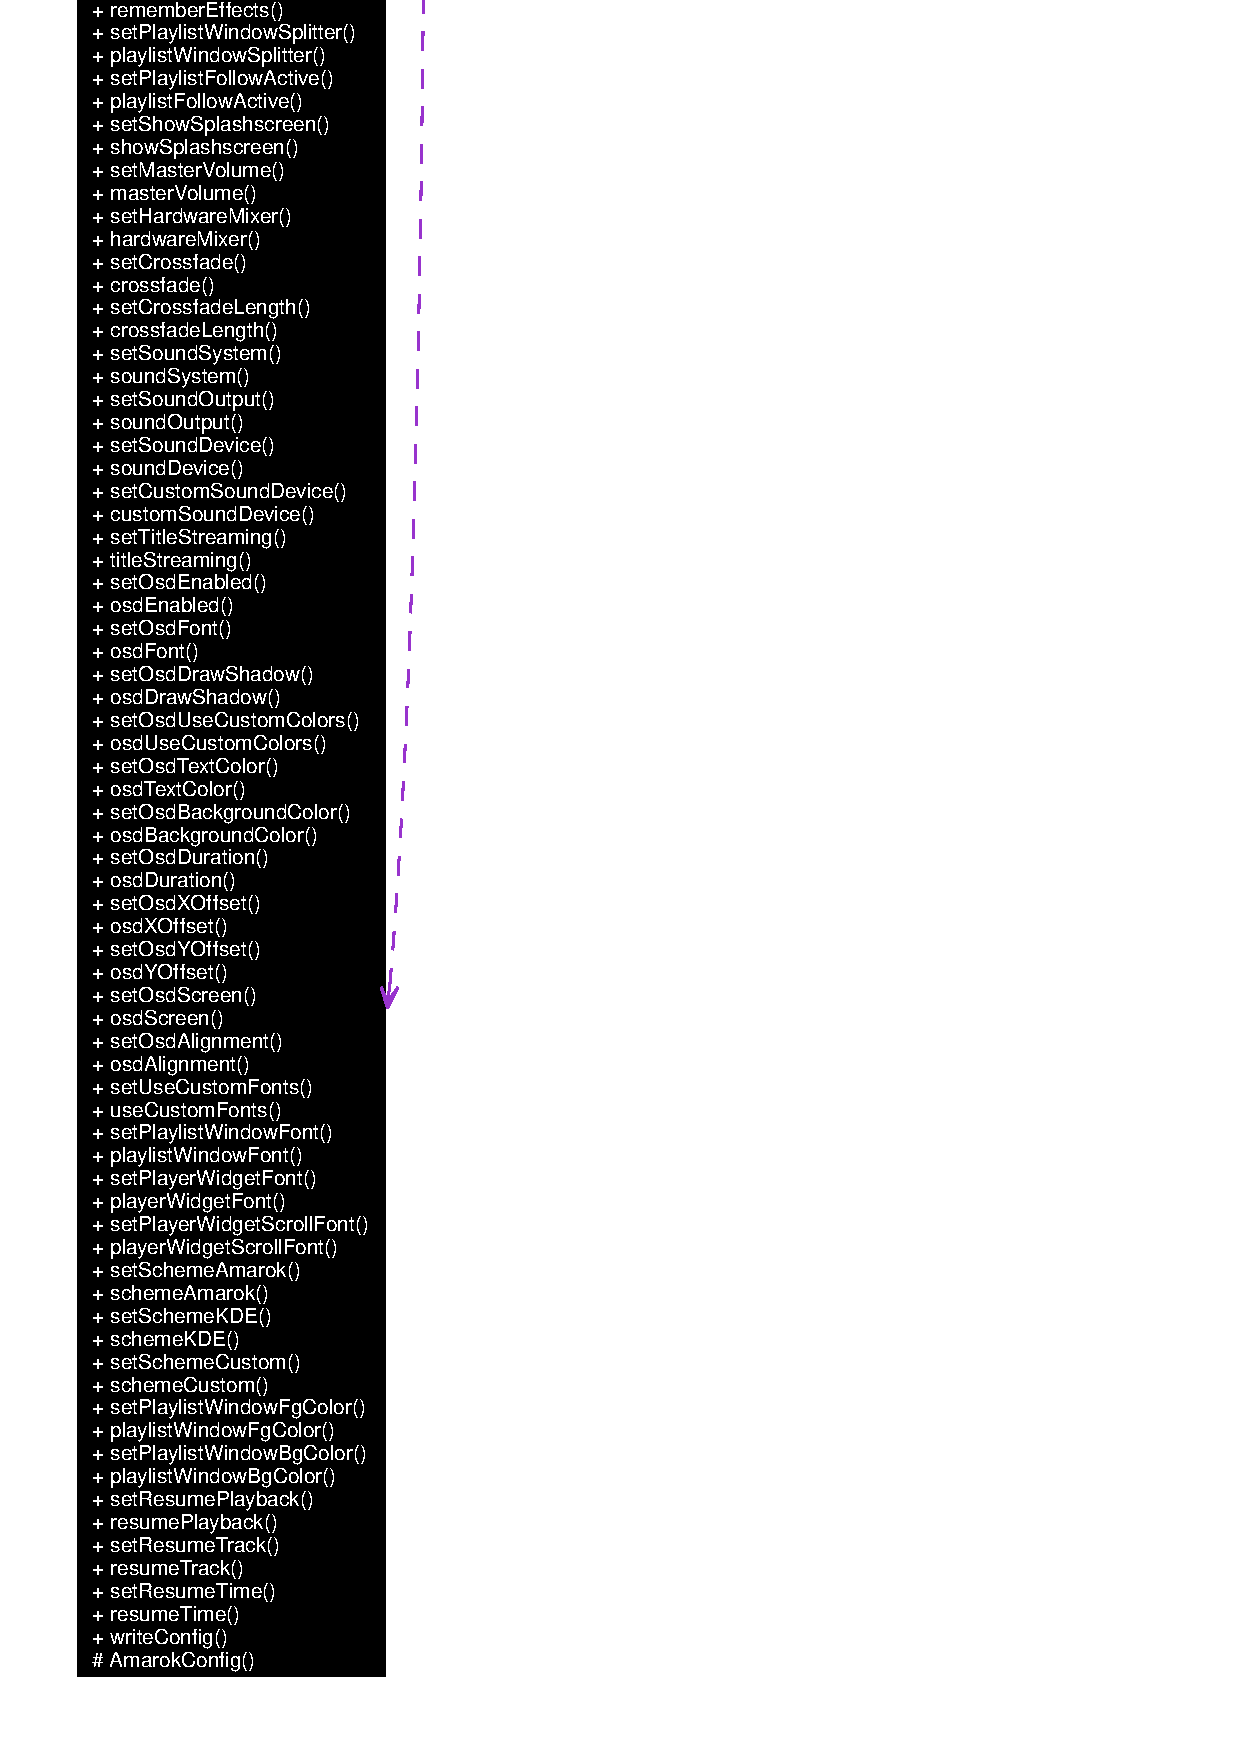
\includegraphics[width=115pt]{classAmarokConfig__coll__graph}
\end{center}
\end{figure}
\subsection*{Public Member Functions}
\begin{CompactItemize}
\item 
{\bf $\sim$Amarok\-Config} ()
\end{CompactItemize}
\subsection*{Static Public Member Functions}
\begin{CompactItemize}
\item 
{\bf Amarok\-Config} $\ast$ {\bf self} ()
\item 
void {\bf set\-Version} (const QString \&v)
\item 
QString {\bf version} ()
\item 
void {\bf set\-Player\-Pos} (const QPoint \&v)
\item 
QPoint {\bf player\-Pos} ()
\item 
void {\bf set\-Playlist\-Window\-Pos} (const QPoint \&v)
\item 
QPoint {\bf playlist\-Window\-Pos} ()
\item 
void {\bf set\-Playlist\-Window\-Size} (const QSize \&v)
\item 
QSize {\bf playlist\-Window\-Size} ()
\item 
void {\bf set\-Save\-Playlist} (bool v)
\item 
bool {\bf save\-Playlist} ()
\item 
void {\bf set\-Follow\-Symlinks} (bool v)
\item 
bool {\bf follow\-Symlinks} ()
\item 
void {\bf set\-Time\-Display\-Remaining} (bool v)
\item 
bool {\bf time\-Display\-Remaining} ()
\item 
void {\bf set\-Repeat\-Track} (bool v)
\item 
bool {\bf repeat\-Track} ()
\item 
void {\bf set\-Repeat\-Playlist} (bool v)
\item 
bool {\bf repeat\-Playlist} ()
\item 
void {\bf set\-Random\-Mode} (bool v)
\item 
bool {\bf random\-Mode} ()
\item 
void {\bf set\-Show\-Meta\-Info} (bool v)
\item 
bool {\bf show\-Meta\-Info} ()
\item 
void {\bf set\-Show\-Tray\-Icon} (bool v)
\item 
bool {\bf show\-Tray\-Icon} ()
\item 
void {\bf set\-Show\-Player\-Window} (bool v)
\item 
bool {\bf show\-Player\-Window} ()
\item 
void {\bf set\-Show\-Status\-Bar} (bool v)
\item 
bool {\bf show\-Status\-Bar} ()
\item 
void {\bf set\-Show\-Welcome\-Tab} (bool v)
\item 
bool {\bf show\-Welcome\-Tab} ()
\item 
void {\bf set\-Directories\-Recursively} (bool v)
\item 
bool {\bf directories\-Recursively} ()
\item 
void {\bf set\-Track\-Delay\-Length} (int v)
\item 
int {\bf track\-Delay\-Length} ()
\item 
void {\bf set\-Hide\-Playlist\-Window} (bool v)
\item 
bool {\bf hide\-Playlist\-Window} ()
\item 
void {\bf set\-Playlist\-Window\-Enabled} (bool v)
\item 
bool {\bf playlist\-Window\-Enabled} ()
\item 
void {\bf set\-Undo\-Levels} (int v)
\item 
int {\bf undo\-Levels} ()
\item 
void {\bf set\-Current\-Analyzer} (int v)
\item 
int {\bf current\-Analyzer} ()
\item 
void {\bf set\-Remember\-Effects} (bool v)
\item 
bool {\bf remember\-Effects} ()
\item 
void {\bf set\-Playlist\-Window\-Splitter} (const QValue\-List$<$ int $>$ \&v)
\item 
QValue\-List$<$ int $>$ {\bf playlist\-Window\-Splitter} ()
\item 
void {\bf set\-Playlist\-Follow\-Active} (bool v)
\item 
bool {\bf playlist\-Follow\-Active} ()
\item 
void {\bf set\-Show\-Splashscreen} (bool v)
\item 
bool {\bf show\-Splashscreen} ()
\item 
void {\bf set\-Master\-Volume} (int v)
\item 
int {\bf master\-Volume} ()
\item 
void {\bf set\-Hardware\-Mixer} (bool v)
\item 
bool {\bf hardware\-Mixer} ()
\item 
void {\bf set\-Crossfade} (bool v)
\item 
bool {\bf crossfade} ()
\item 
void {\bf set\-Crossfade\-Length} (int v)
\item 
int {\bf crossfade\-Length} ()
\item 
void {\bf set\-Sound\-System} (const QString \&v)
\item 
QString {\bf sound\-System} ()
\item 
void {\bf set\-Sound\-Output} (const QString \&v)
\item 
QString {\bf sound\-Output} ()
\item 
void {\bf set\-Sound\-Device} (const QString \&v)
\item 
QString {\bf sound\-Device} ()
\item 
void {\bf set\-Custom\-Sound\-Device} (bool v)
\item 
bool {\bf custom\-Sound\-Device} ()
\item 
void {\bf set\-Title\-Streaming} (bool v)
\item 
bool {\bf title\-Streaming} ()
\item 
void {\bf set\-Osd\-Enabled} (bool v)
\item 
bool {\bf osd\-Enabled} ()
\item 
void {\bf set\-Osd\-Font} (const QFont \&v)
\item 
QFont {\bf osd\-Font} ()
\item 
void {\bf set\-Osd\-Draw\-Shadow} (bool v)
\item 
bool {\bf osd\-Draw\-Shadow} ()
\item 
void {\bf set\-Osd\-Use\-Custom\-Colors} (bool v)
\item 
bool {\bf osd\-Use\-Custom\-Colors} ()
\item 
void {\bf set\-Osd\-Text\-Color} (const QColor \&v)
\item 
QColor {\bf osd\-Text\-Color} ()
\item 
void {\bf set\-Osd\-Background\-Color} (const QColor \&v)
\item 
QColor {\bf osd\-Background\-Color} ()
\item 
void {\bf set\-Osd\-Duration} (int v)
\item 
int {\bf osd\-Duration} ()
\item 
void {\bf set\-Osd\-XOffset} (int v)
\item 
int {\bf osd\-XOffset} ()
\item 
void {\bf set\-Osd\-YOffset} (int v)
\item 
int {\bf osd\-YOffset} ()
\item 
void {\bf set\-Osd\-Screen} (int v)
\item 
int {\bf osd\-Screen} ()
\item 
void {\bf set\-Osd\-Alignment} (int v)
\item 
int {\bf osd\-Alignment} ()
\item 
void {\bf set\-Use\-Custom\-Fonts} (bool v)
\item 
bool {\bf use\-Custom\-Fonts} ()
\item 
void {\bf set\-Playlist\-Window\-Font} (const QFont \&v)
\item 
QFont {\bf playlist\-Window\-Font} ()
\item 
void {\bf set\-Player\-Widget\-Font} (const QFont \&v)
\item 
QFont {\bf player\-Widget\-Font} ()
\item 
void {\bf set\-Player\-Widget\-Scroll\-Font} (const QFont \&v)
\item 
QFont {\bf player\-Widget\-Scroll\-Font} ()
\item 
void {\bf set\-Scheme\-Amarok} (bool v)
\item 
bool {\bf scheme\-Amarok} ()
\item 
void {\bf set\-Scheme\-KDE} (bool v)
\item 
bool {\bf scheme\-KDE} ()
\item 
void {\bf set\-Scheme\-Custom} (bool v)
\item 
bool {\bf scheme\-Custom} ()
\item 
void {\bf set\-Playlist\-Window\-Fg\-Color} (const QColor \&v)
\item 
QColor {\bf playlist\-Window\-Fg\-Color} ()
\item 
void {\bf set\-Playlist\-Window\-Bg\-Color} (const QColor \&v)
\item 
QColor {\bf playlist\-Window\-Bg\-Color} ()
\item 
void {\bf set\-Resume\-Playback} (bool v)
\item 
bool {\bf resume\-Playback} ()
\item 
void {\bf set\-Resume\-Track} (const QString \&v)
\item 
QString {\bf resume\-Track} ()
\item 
void {\bf set\-Resume\-Time} (int v)
\item 
int {\bf resume\-Time} ()
\item 
void {\bf write\-Config} ()
\end{CompactItemize}
\subsection*{Protected Member Functions}
\begin{CompactItemize}
\item 
{\bf Amarok\-Config} ()
\end{CompactItemize}
\subsection*{Protected Attributes}
\begin{CompactItemize}
\item 
QString {\bf m\-Version}
\item 
QPoint {\bf m\-Player\-Pos}
\item 
QPoint {\bf m\-Playlist\-Window\-Pos}
\item 
QSize {\bf m\-Playlist\-Window\-Size}
\item 
bool {\bf m\-Save\-Playlist}
\item 
bool {\bf m\-Follow\-Symlinks}
\item 
bool {\bf m\-Time\-Display\-Remaining}
\item 
bool {\bf m\-Repeat\-Track}
\item 
bool {\bf m\-Repeat\-Playlist}
\item 
bool {\bf m\-Random\-Mode}
\item 
bool {\bf m\-Show\-Meta\-Info}
\item 
bool {\bf m\-Show\-Tray\-Icon}
\item 
bool {\bf m\-Show\-Player\-Window}
\item 
bool {\bf m\-Show\-Status\-Bar}
\item 
bool {\bf m\-Show\-Welcome\-Tab}
\item 
bool {\bf m\-Directories\-Recursively}
\item 
int {\bf m\-Track\-Delay\-Length}
\item 
bool {\bf m\-Hide\-Playlist\-Window}
\item 
bool {\bf m\-Playlist\-Window\-Enabled}
\item 
int {\bf m\-Undo\-Levels}
\item 
int {\bf m\-Current\-Analyzer}
\item 
bool {\bf m\-Remember\-Effects}
\item 
QValue\-List$<$ int $>$ {\bf m\-Playlist\-Window\-Splitter}
\item 
bool {\bf m\-Playlist\-Follow\-Active}
\item 
bool {\bf m\-Show\-Splashscreen}
\item 
int {\bf m\-Master\-Volume}
\item 
bool {\bf m\-Hardware\-Mixer}
\item 
bool {\bf m\-Crossfade}
\item 
int {\bf m\-Crossfade\-Length}
\item 
QString {\bf m\-Sound\-System}
\item 
QString {\bf m\-Sound\-Output}
\item 
QString {\bf m\-Sound\-Device}
\item 
bool {\bf m\-Custom\-Sound\-Device}
\item 
bool {\bf m\-Title\-Streaming}
\item 
bool {\bf m\-Osd\-Enabled}
\item 
QFont {\bf m\-Osd\-Font}
\item 
bool {\bf m\-Osd\-Draw\-Shadow}
\item 
bool {\bf m\-Osd\-Use\-Custom\-Colors}
\item 
QColor {\bf m\-Osd\-Text\-Color}
\item 
QColor {\bf m\-Osd\-Background\-Color}
\item 
int {\bf m\-Osd\-Duration}
\item 
int {\bf m\-Osd\-XOffset}
\item 
int {\bf m\-Osd\-YOffset}
\item 
int {\bf m\-Osd\-Screen}
\item 
int {\bf m\-Osd\-Alignment}
\item 
bool {\bf m\-Use\-Custom\-Fonts}
\item 
QFont {\bf m\-Playlist\-Window\-Font}
\item 
QFont {\bf m\-Player\-Widget\-Font}
\item 
QFont {\bf m\-Player\-Widget\-Scroll\-Font}
\item 
bool {\bf m\-Scheme\-Amarok}
\item 
bool {\bf m\-Scheme\-KDE}
\item 
bool {\bf m\-Scheme\-Custom}
\item 
QColor {\bf m\-Playlist\-Window\-Fg\-Color}
\item 
QColor {\bf m\-Playlist\-Window\-Bg\-Color}
\item 
bool {\bf m\-Resume\-Playback}
\item 
QString {\bf m\-Resume\-Track}
\item 
int {\bf m\-Resume\-Time}
\end{CompactItemize}
\subsection*{Static Protected Attributes}
\begin{CompactItemize}
\item 
{\bf Amarok\-Config} $\ast$ {\bf m\-Self} = 0
\end{CompactItemize}


\subsection{Constructor \& Destructor Documentation}
\index{AmarokConfig@{Amarok\-Config}!~AmarokConfig@{$\sim$AmarokConfig}}
\index{~AmarokConfig@{$\sim$AmarokConfig}!AmarokConfig@{Amarok\-Config}}
\subsubsection{\setlength{\rightskip}{0pt plus 5cm}Amarok\-Config::$\sim${\bf Amarok\-Config} ()}\label{classAmarokConfig_AmarokConfiga0}




Definition at line 249 of file amarokconfig.cpp.

References m\-Self, and static\-Deleter.



\footnotesize\begin{verbatim}250 {
251   if ( mSelf == this )
252     staticDeleter.setObject( mSelf, 0, false );
253 }
\end{verbatim}\normalsize 
\index{AmarokConfig@{Amarok\-Config}!AmarokConfig@{AmarokConfig}}
\index{AmarokConfig@{AmarokConfig}!AmarokConfig@{Amarok\-Config}}
\subsubsection{\setlength{\rightskip}{0pt plus 5cm}Amarok\-Config::Amarok\-Config ()\hspace{0.3cm}{\tt  [protected]}}\label{classAmarokConfig_AmarokConfigb0}




Definition at line 22 of file amarokconfig.cpp.

References m\-Crossfade, m\-Crossfade\-Length, m\-Current\-Analyzer, m\-Custom\-Sound\-Device, m\-Directories\-Recursively, m\-Follow\-Symlinks, m\-Hardware\-Mixer, m\-Hide\-Playlist\-Window, m\-Master\-Volume, m\-Osd\-Alignment, m\-Osd\-Background\-Color, m\-Osd\-Draw\-Shadow, m\-Osd\-Duration, m\-Osd\-Enabled, m\-Osd\-Font, m\-Osd\-Screen, m\-Osd\-Text\-Color, m\-Osd\-Use\-Custom\-Colors, m\-Osd\-XOffset, m\-Osd\-YOffset, m\-Player\-Pos, m\-Player\-Widget\-Font, m\-Player\-Widget\-Scroll\-Font, m\-Playlist\-Follow\-Active, m\-Playlist\-Window\-Bg\-Color, m\-Playlist\-Window\-Enabled, m\-Playlist\-Window\-Fg\-Color, m\-Playlist\-Window\-Font, m\-Playlist\-Window\-Pos, m\-Playlist\-Window\-Size, m\-Playlist\-Window\-Splitter, m\-Random\-Mode, m\-Remember\-Effects, m\-Repeat\-Playlist, m\-Repeat\-Track, m\-Resume\-Playback, m\-Resume\-Time, m\-Resume\-Track, m\-Save\-Playlist, m\-Scheme\-Amarok, m\-Scheme\-Custom, m\-Scheme\-KDE, m\-Self, m\-Show\-Meta\-Info, m\-Show\-Player\-Window, m\-Show\-Splashscreen, m\-Show\-Status\-Bar, m\-Show\-Tray\-Icon, m\-Show\-Welcome\-Tab, m\-Sound\-Device, m\-Sound\-Output, m\-Sound\-System, m\-Time\-Display\-Remaining, m\-Title\-Streaming, m\-Track\-Delay\-Length, m\-Undo\-Levels, m\-Use\-Custom\-Fonts, and m\-Version.

Referenced by self().



\footnotesize\begin{verbatim}23   : KConfigSkeleton( "amarokrc" )
24 {
25   mSelf = this;
26   setCurrentGroup( "General Options" );
27 
28   KConfigSkeleton::ItemString  *itemVersion;
29   itemVersion = new KConfigSkeleton::ItemString( currentGroup(), "Version", mVersion );
30   addItem( itemVersion );
31   KConfigSkeleton::ItemPoint  *itemPlayerPos;
32   itemPlayerPos = new KConfigSkeleton::ItemPoint( currentGroup(), "Player Pos", mPlayerPos, QPoint(-1,-1) );
33   addItem( itemPlayerPos, "PlayerPos" );
34   KConfigSkeleton::ItemPoint  *itemPlaylistWindowPos;
35   itemPlaylistWindowPos = new KConfigSkeleton::ItemPoint( currentGroup(), "Playlist Window Pos", mPlaylistWindowPos, QPoint(-1,-1) );
36   addItem( itemPlaylistWindowPos, "PlaylistWindowPos" );
37   KConfigSkeleton::ItemSize  *itemPlaylistWindowSize;
38   itemPlaylistWindowSize = new KConfigSkeleton::ItemSize( currentGroup(), "Playlist Window Size", mPlaylistWindowSize, QSize(600,450) );
39   addItem( itemPlaylistWindowSize, "PlaylistWindowSize" );
40   KConfigSkeleton::ItemBool  *itemSavePlaylist;
41   itemSavePlaylist = new KConfigSkeleton::ItemBool( currentGroup(), "Save Playlist", mSavePlaylist, true );
42   addItem( itemSavePlaylist, "SavePlaylist" );
43   KConfigSkeleton::ItemBool  *itemFollowSymlinks;
44   itemFollowSymlinks = new KConfigSkeleton::ItemBool( currentGroup(), "Follow Symlinks", mFollowSymlinks, true );
45   addItem( itemFollowSymlinks, "FollowSymlinks" );
46   KConfigSkeleton::ItemBool  *itemTimeDisplayRemaining;
47   itemTimeDisplayRemaining = new KConfigSkeleton::ItemBool( currentGroup(), "Time Display Remaining", mTimeDisplayRemaining, false );
48   addItem( itemTimeDisplayRemaining, "TimeDisplayRemaining" );
49   KConfigSkeleton::ItemBool  *itemRepeatTrack;
50   itemRepeatTrack = new KConfigSkeleton::ItemBool( currentGroup(), "Repeat Track", mRepeatTrack, false );
51   addItem( itemRepeatTrack, "RepeatTrack" );
52   KConfigSkeleton::ItemBool  *itemRepeatPlaylist;
53   itemRepeatPlaylist = new KConfigSkeleton::ItemBool( currentGroup(), "Repeat Playlist", mRepeatPlaylist, false );
54   addItem( itemRepeatPlaylist, "RepeatPlaylist" );
55   KConfigSkeleton::ItemBool  *itemRandomMode;
56   itemRandomMode = new KConfigSkeleton::ItemBool( currentGroup(), "Random Mode", mRandomMode, false );
57   addItem( itemRandomMode, "RandomMode" );
58   KConfigSkeleton::ItemBool  *itemShowMetaInfo;
59   itemShowMetaInfo = new KConfigSkeleton::ItemBool( currentGroup(), "Show Meta Info", mShowMetaInfo, true );
60   addItem( itemShowMetaInfo, "ShowMetaInfo" );
61   KConfigSkeleton::ItemBool  *itemShowTrayIcon;
62   itemShowTrayIcon = new KConfigSkeleton::ItemBool( currentGroup(), "Show Tray Icon", mShowTrayIcon, true );
63   addItem( itemShowTrayIcon, "ShowTrayIcon" );
64   KConfigSkeleton::ItemBool  *itemShowPlayerWindow;
65   itemShowPlayerWindow = new KConfigSkeleton::ItemBool( currentGroup(), "Show Player Window", mShowPlayerWindow, true );
66   addItem( itemShowPlayerWindow, "ShowPlayerWindow" );
67   KConfigSkeleton::ItemBool  *itemShowStatusBar;
68   itemShowStatusBar = new KConfigSkeleton::ItemBool( currentGroup(), "Show Status Bar", mShowStatusBar, false );
69   addItem( itemShowStatusBar, "ShowStatusBar" );
70   KConfigSkeleton::ItemBool  *itemShowWelcomeTab;
71   itemShowWelcomeTab = new KConfigSkeleton::ItemBool( currentGroup(), "Show Welcome Tab", mShowWelcomeTab, true );
72   addItem( itemShowWelcomeTab, "ShowWelcomeTab" );
73   KConfigSkeleton::ItemBool  *itemDirectoriesRecursively;
74   itemDirectoriesRecursively = new KConfigSkeleton::ItemBool( currentGroup(), "Directories Recursively", mDirectoriesRecursively, true );
75   addItem( itemDirectoriesRecursively, "DirectoriesRecursively" );
76   KConfigSkeleton::ItemInt  *itemTrackDelayLength;
77   itemTrackDelayLength = new KConfigSkeleton::ItemInt( currentGroup(), "Track Delay Length", mTrackDelayLength, 0 );
78   addItem( itemTrackDelayLength, "TrackDelayLength" );
79   KConfigSkeleton::ItemBool  *itemHidePlaylistWindow;
80   itemHidePlaylistWindow = new KConfigSkeleton::ItemBool( currentGroup(), "Hide Playlist Window", mHidePlaylistWindow, true );
81   addItem( itemHidePlaylistWindow, "HidePlaylistWindow" );
82   KConfigSkeleton::ItemBool  *itemPlaylistWindowEnabled;
83   itemPlaylistWindowEnabled = new KConfigSkeleton::ItemBool( currentGroup(), "Playlist Window Enabled", mPlaylistWindowEnabled, true );
84   addItem( itemPlaylistWindowEnabled, "PlaylistWindowEnabled" );
85   KConfigSkeleton::ItemInt  *itemUndoLevels;
86   itemUndoLevels = new KConfigSkeleton::ItemInt( currentGroup(), "Undo Levels", mUndoLevels, 30 );
87   addItem( itemUndoLevels, "UndoLevels" );
88   KConfigSkeleton::ItemInt  *itemCurrentAnalyzer;
89   itemCurrentAnalyzer = new KConfigSkeleton::ItemInt( currentGroup(), "Current Analyzer", mCurrentAnalyzer, -1 );
90   addItem( itemCurrentAnalyzer, "CurrentAnalyzer" );
91   KConfigSkeleton::ItemBool  *itemRememberEffects;
92   itemRememberEffects = new KConfigSkeleton::ItemBool( currentGroup(), "Remember Effects", mRememberEffects, true );
93   addItem( itemRememberEffects, "RememberEffects" );
94   QValueList<int> defaultPlaylistWindowSplitter;
95   defaultPlaylistWindowSplitter.append( 70 );
96   defaultPlaylistWindowSplitter.append( 140 );
97 
98   KConfigSkeleton::ItemIntList  *itemPlaylistWindowSplitter;
99   itemPlaylistWindowSplitter = new KConfigSkeleton::ItemIntList( currentGroup(), "Playlist Window Splitter", mPlaylistWindowSplitter, defaultPlaylistWindowSplitter );
100   addItem( itemPlaylistWindowSplitter, "PlaylistWindowSplitter" );
101   KConfigSkeleton::ItemBool  *itemPlaylistFollowActive;
102   itemPlaylistFollowActive = new KConfigSkeleton::ItemBool( currentGroup(), "Playlist Follow Active", mPlaylistFollowActive, false );
103   addItem( itemPlaylistFollowActive, "PlaylistFollowActive" );
104   KConfigSkeleton::ItemBool  *itemShowSplashscreen;
105   itemShowSplashscreen = new KConfigSkeleton::ItemBool( currentGroup(), "Show Splashscreen", mShowSplashscreen, true );
106   addItem( itemShowSplashscreen, "ShowSplashscreen" );
107 
108   setCurrentGroup( "Playback" );
109 
110   KConfigSkeleton::ItemInt  *itemMasterVolume;
111   itemMasterVolume = new KConfigSkeleton::ItemInt( currentGroup(), "Master Volume", mMasterVolume, 50 );
112   itemMasterVolume->setMinValue(0);
113   itemMasterVolume->setMaxValue(100);
114   addItem( itemMasterVolume, "MasterVolume" );
115   KConfigSkeleton::ItemBool  *itemHardwareMixer;
116   itemHardwareMixer = new KConfigSkeleton::ItemBool( currentGroup(), "Hardware Mixer", mHardwareMixer, false );
117   addItem( itemHardwareMixer, "HardwareMixer" );
118   KConfigSkeleton::ItemBool  *itemCrossfade;
119   itemCrossfade = new KConfigSkeleton::ItemBool( currentGroup(), "Crossfade", mCrossfade, true );
120   addItem( itemCrossfade );
121   KConfigSkeleton::ItemInt  *itemCrossfadeLength;
122   itemCrossfadeLength = new KConfigSkeleton::ItemInt( currentGroup(), "Crossfade Length", mCrossfadeLength, 2200 );
123   addItem( itemCrossfadeLength, "CrossfadeLength" );
124   KConfigSkeleton::ItemString  *itemSoundSystem;
125   itemSoundSystem = new KConfigSkeleton::ItemString( currentGroup(), "Sound System", mSoundSystem, "aRts Engine" );
126   addItem( itemSoundSystem, "SoundSystem" );
127   KConfigSkeleton::ItemString  *itemSoundOutput;
128   itemSoundOutput = new KConfigSkeleton::ItemString( currentGroup(), "Sound Output", mSoundOutput, "Alsa" );
129   addItem( itemSoundOutput, "SoundOutput" );
130   KConfigSkeleton::ItemString  *itemSoundDevice;
131   itemSoundDevice = new KConfigSkeleton::ItemString( currentGroup(), "Sound Device", mSoundDevice );
132   addItem( itemSoundDevice, "SoundDevice" );
133   KConfigSkeleton::ItemBool  *itemCustomSoundDevice;
134   itemCustomSoundDevice = new KConfigSkeleton::ItemBool( currentGroup(), "Custom Sound Device", mCustomSoundDevice, false );
135   addItem( itemCustomSoundDevice, "CustomSoundDevice" );
136   KConfigSkeleton::ItemBool  *itemTitleStreaming;
137   itemTitleStreaming = new KConfigSkeleton::ItemBool( currentGroup(), "Title Streaming", mTitleStreaming, true );
138   addItem( itemTitleStreaming, "TitleStreaming" );
139 
140   setCurrentGroup( "OSD" );
141 
142   KConfigSkeleton::ItemBool  *itemOsdEnabled;
143   itemOsdEnabled = new KConfigSkeleton::ItemBool( currentGroup(), "Osd Enabled", mOsdEnabled, true );
144   addItem( itemOsdEnabled, "OsdEnabled" );
145   KConfigSkeleton::ItemFont  *itemOsdFont;
146   itemOsdFont = new KConfigSkeleton::ItemFont( currentGroup(), "Osd Font", mOsdFont, QFont("Arial",20) );
147   addItem( itemOsdFont, "OsdFont" );
148   KConfigSkeleton::ItemBool  *itemOsdDrawShadow;
149   itemOsdDrawShadow = new KConfigSkeleton::ItemBool( currentGroup(), "Osd Draw Shadow", mOsdDrawShadow, true );
150   addItem( itemOsdDrawShadow, "OsdDrawShadow" );
151   KConfigSkeleton::ItemBool  *itemOsdUseCustomColors;
152   itemOsdUseCustomColors = new KConfigSkeleton::ItemBool( currentGroup(), "Osd Use Custom Colors", mOsdUseCustomColors, false );
153   addItem( itemOsdUseCustomColors, "OsdUseCustomColors" );
154   KConfigSkeleton::ItemColor  *itemOsdTextColor;
155   itemOsdTextColor = new KConfigSkeleton::ItemColor( currentGroup(), "Osd Text Color", mOsdTextColor, QColor( "#ffff00" ) );
156   addItem( itemOsdTextColor, "OsdTextColor" );
157   KConfigSkeleton::ItemColor  *itemOsdBackgroundColor;
158   itemOsdBackgroundColor = new KConfigSkeleton::ItemColor( currentGroup(), "Osd Background Color", mOsdBackgroundColor, QColor( "#1500a0" ) );
159   addItem( itemOsdBackgroundColor, "OsdBackgroundColor" );
160   KConfigSkeleton::ItemInt  *itemOsdDuration;
161   itemOsdDuration = new KConfigSkeleton::ItemInt( currentGroup(), "Osd Duration", mOsdDuration, 5000 );
162   itemOsdDuration->setMinValue(500);
163   itemOsdDuration->setMaxValue(10000);
164   addItem( itemOsdDuration, "OsdDuration" );
165   KConfigSkeleton::ItemInt  *itemOsdXOffset;
166   itemOsdXOffset = new KConfigSkeleton::ItemInt( currentGroup(), "Osd X Offset", mOsdXOffset, 30 );
167   itemOsdXOffset->setMinValue(0);
168   itemOsdXOffset->setMaxValue(10000);
169   addItem( itemOsdXOffset, "OsdXOffset" );
170   KConfigSkeleton::ItemInt  *itemOsdYOffset;
171   itemOsdYOffset = new KConfigSkeleton::ItemInt( currentGroup(), "Osd Y Offset", mOsdYOffset, 30 );
172   itemOsdYOffset->setMinValue(0);
173   itemOsdYOffset->setMaxValue(10000);
174   addItem( itemOsdYOffset, "OsdYOffset" );
175   KConfigSkeleton::ItemInt  *itemOsdScreen;
176   itemOsdScreen = new KConfigSkeleton::ItemInt( currentGroup(), "Osd Screen", mOsdScreen, 0 );
177   addItem( itemOsdScreen, "OsdScreen" );
178   QValueList<KConfigSkeleton::ItemEnum::Choice> valuesOsdAlignment;
179   {
180     KConfigSkeleton::ItemEnum::Choice choice;
181     choice.name = "Left";
182     valuesOsdAlignment.append( choice );
183   }
184   {
185     KConfigSkeleton::ItemEnum::Choice choice;
186     choice.name = "Middle";
187     valuesOsdAlignment.append( choice );
188   }
189   {
190     KConfigSkeleton::ItemEnum::Choice choice;
191     choice.name = "Center";
192     valuesOsdAlignment.append( choice );
193   }
194   {
195     KConfigSkeleton::ItemEnum::Choice choice;
196     choice.name = "Right";
197     valuesOsdAlignment.append( choice );
198   }
199   KConfigSkeleton::ItemEnum  *itemOsdAlignment;
200   itemOsdAlignment = new KConfigSkeleton::ItemEnum( currentGroup(), "Osd Alignment", mOsdAlignment, valuesOsdAlignment, EnumOsdAlignment::Center );
201   addItem( itemOsdAlignment, "OsdAlignment" );
202 
203   setCurrentGroup( "Fonts" );
204 
205   KConfigSkeleton::ItemBool  *itemUseCustomFonts;
206   itemUseCustomFonts = new KConfigSkeleton::ItemBool( currentGroup(), "Use Custom Fonts", mUseCustomFonts, false );
207   addItem( itemUseCustomFonts, "UseCustomFonts" );
208   KConfigSkeleton::ItemFont  *itemPlaylistWindowFont;
209   itemPlaylistWindowFont = new KConfigSkeleton::ItemFont( currentGroup(), "Playlist Window Font", mPlaylistWindowFont, QFont("Helvetica",9) );
210   addItem( itemPlaylistWindowFont, "PlaylistWindowFont" );
211   KConfigSkeleton::ItemFont  *itemPlayerWidgetFont;
212   itemPlayerWidgetFont = new KConfigSkeleton::ItemFont( currentGroup(), "Player Widget Font", mPlayerWidgetFont, QFont("Helvetica",9) );
213   addItem( itemPlayerWidgetFont, "PlayerWidgetFont" );
214   KConfigSkeleton::ItemFont  *itemPlayerWidgetScrollFont;
215   itemPlayerWidgetScrollFont = new KConfigSkeleton::ItemFont( currentGroup(), "Player Widget Scroll Font", mPlayerWidgetScrollFont, QFont("Helvetica",9) );
216   addItem( itemPlayerWidgetScrollFont, "PlayerWidgetScrollFont" );
217 
218   setCurrentGroup( "Colors" );
219 
220   KConfigSkeleton::ItemBool  *itemSchemeAmarok;
221   itemSchemeAmarok = new KConfigSkeleton::ItemBool( currentGroup(), "Scheme Amarok", mSchemeAmarok, false );
222   addItem( itemSchemeAmarok, "SchemeAmarok" );
223   KConfigSkeleton::ItemBool  *itemSchemeKDE;
224   itemSchemeKDE = new KConfigSkeleton::ItemBool( currentGroup(), "Scheme KDE", mSchemeKDE, true );
225   addItem( itemSchemeKDE, "SchemeKDE" );
226   KConfigSkeleton::ItemBool  *itemSchemeCustom;
227   itemSchemeCustom = new KConfigSkeleton::ItemBool( currentGroup(), "Scheme Custom", mSchemeCustom, false );
228   addItem( itemSchemeCustom, "SchemeCustom" );
229   KConfigSkeleton::ItemColor  *itemPlaylistWindowFgColor;
230   itemPlaylistWindowFgColor = new KConfigSkeleton::ItemColor( currentGroup(), "Playlist Window Fg Color", mPlaylistWindowFgColor, QColor( "#80a0ff" ) );
231   addItem( itemPlaylistWindowFgColor, "PlaylistWindowFgColor" );
232   KConfigSkeleton::ItemColor  *itemPlaylistWindowBgColor;
233   itemPlaylistWindowBgColor = new KConfigSkeleton::ItemColor( currentGroup(), "Playlist Window Bg Color", mPlaylistWindowBgColor, QColor( "#000000" ) );
234   addItem( itemPlaylistWindowBgColor, "PlaylistWindowBgColor" );
235 
236   setCurrentGroup( "Session" );
237 
238   KConfigSkeleton::ItemBool  *itemResumePlayback;
239   itemResumePlayback = new KConfigSkeleton::ItemBool( currentGroup(), "Resume Playback", mResumePlayback, false );
240   addItem( itemResumePlayback, "ResumePlayback" );
241   KConfigSkeleton::ItemPath  *itemResumeTrack;
242   itemResumeTrack = new KConfigSkeleton::ItemPath( currentGroup(), "Resume Track", mResumeTrack );
243   addItem( itemResumeTrack, "ResumeTrack" );
244   KConfigSkeleton::ItemInt  *itemResumeTime;
245   itemResumeTime = new KConfigSkeleton::ItemInt( currentGroup(), "Resume Time", mResumeTime, -1 );
246   addItem( itemResumeTime, "ResumeTime" );
247 }
\end{verbatim}\normalsize 


\subsection{Member Function Documentation}
\index{AmarokConfig@{Amarok\-Config}!crossfade@{crossfade}}
\index{crossfade@{crossfade}!AmarokConfig@{Amarok\-Config}}
\subsubsection{\setlength{\rightskip}{0pt plus 5cm}bool Amarok\-Config::crossfade ()\hspace{0.3cm}{\tt  [inline, static]}}\label{classAmarokConfig_AmarokConfige56}


Get Whether to crossfade between tracks 

Definition at line 547 of file amarokconfig.h.

References m\-Crossfade, and self().

Referenced by Engine\-Controller::slot\-Main\-Timer().



\footnotesize\begin{verbatim}548     {
549       return self()->mCrossfade;
550     }
\end{verbatim}\normalsize 


Here is the call graph for this function:\begin{figure}[H]
\begin{center}
\leavevmode
\includegraphics[width=245pt]{classAmarokConfig_AmarokConfige56_cgraph}
\end{center}
\end{figure}
\index{AmarokConfig@{Amarok\-Config}!crossfadeLength@{crossfadeLength}}
\index{crossfadeLength@{crossfadeLength}!AmarokConfig@{Amarok\-Config}}
\subsubsection{\setlength{\rightskip}{0pt plus 5cm}int Amarok\-Config::crossfade\-Length ()\hspace{0.3cm}{\tt  [inline, static]}}\label{classAmarokConfig_AmarokConfige58}


Get Length of crossfade, in milliseconds 

Definition at line 566 of file amarokconfig.h.

References m\-Crossfade\-Length, and self().

Referenced by Engine\-Controller::slot\-Main\-Timer().



\footnotesize\begin{verbatim}567     {
568       return self()->mCrossfadeLength;
569     }
\end{verbatim}\normalsize 


Here is the call graph for this function:\begin{figure}[H]
\begin{center}
\leavevmode
\includegraphics[width=261pt]{classAmarokConfig_AmarokConfige58_cgraph}
\end{center}
\end{figure}
\index{AmarokConfig@{Amarok\-Config}!currentAnalyzer@{currentAnalyzer}}
\index{currentAnalyzer@{currentAnalyzer}!AmarokConfig@{Amarok\-Config}}
\subsubsection{\setlength{\rightskip}{0pt plus 5cm}int Amarok\-Config::current\-Analyzer ()\hspace{0.3cm}{\tt  [inline, static]}}\label{classAmarokConfig_AmarokConfige42}


Get Index of current visual analyzer 

Definition at line 414 of file amarokconfig.h.

References m\-Current\-Analyzer, and self().



\footnotesize\begin{verbatim}415     {
416       return self()->mCurrentAnalyzer;
417     }
\end{verbatim}\normalsize 


Here is the call graph for this function:\begin{figure}[H]
\begin{center}
\leavevmode
\includegraphics[width=259pt]{classAmarokConfig_AmarokConfige42_cgraph}
\end{center}
\end{figure}
\index{AmarokConfig@{Amarok\-Config}!customSoundDevice@{customSoundDevice}}
\index{customSoundDevice@{customSoundDevice}!AmarokConfig@{Amarok\-Config}}
\subsubsection{\setlength{\rightskip}{0pt plus 5cm}bool Amarok\-Config::custom\-Sound\-Device ()\hspace{0.3cm}{\tt  [inline, static]}}\label{classAmarokConfig_AmarokConfige66}


Get Don't use the autodetected audiosink sound device 

Definition at line 642 of file amarokconfig.h.

References m\-Custom\-Sound\-Device, and self().



\footnotesize\begin{verbatim}643     {
644       return self()->mCustomSoundDevice;
645     }
\end{verbatim}\normalsize 


Here is the call graph for this function:\begin{figure}[H]
\begin{center}
\leavevmode
\includegraphics[width=269pt]{classAmarokConfig_AmarokConfige66_cgraph}
\end{center}
\end{figure}
\index{AmarokConfig@{Amarok\-Config}!directoriesRecursively@{directoriesRecursively}}
\index{directoriesRecursively@{directoriesRecursively}!AmarokConfig@{Amarok\-Config}}
\subsubsection{\setlength{\rightskip}{0pt plus 5cm}bool Amarok\-Config::directories\-Recursively ()\hspace{0.3cm}{\tt  [inline, static]}}\label{classAmarokConfig_AmarokConfige32}


Get Whether to add directories to playlist recursively 

Definition at line 319 of file amarokconfig.h.

References m\-Directories\-Recursively, and self().



\footnotesize\begin{verbatim}320     {
321       return self()->mDirectoriesRecursively;
322     }
\end{verbatim}\normalsize 


Here is the call graph for this function:\begin{figure}[H]
\begin{center}
\leavevmode
\includegraphics[width=272pt]{classAmarokConfig_AmarokConfige32_cgraph}
\end{center}
\end{figure}
\index{AmarokConfig@{Amarok\-Config}!followSymlinks@{followSymlinks}}
\index{followSymlinks@{followSymlinks}!AmarokConfig@{Amarok\-Config}}
\subsubsection{\setlength{\rightskip}{0pt plus 5cm}bool Amarok\-Config::follow\-Symlinks ()\hspace{0.3cm}{\tt  [inline, static]}}\label{classAmarokConfig_AmarokConfige12}


Get Whether to follow symlinks while adding items to playlist recursively 

Definition at line 129 of file amarokconfig.h.

References m\-Follow\-Symlinks, and self().



\footnotesize\begin{verbatim}130     {
131       return self()->mFollowSymlinks;
132     }
\end{verbatim}\normalsize 


Here is the call graph for this function:\begin{figure}[H]
\begin{center}
\leavevmode
\includegraphics[width=256pt]{classAmarokConfig_AmarokConfige12_cgraph}
\end{center}
\end{figure}
\index{AmarokConfig@{Amarok\-Config}!hardwareMixer@{hardwareMixer}}
\index{hardwareMixer@{hardwareMixer}!AmarokConfig@{Amarok\-Config}}
\subsubsection{\setlength{\rightskip}{0pt plus 5cm}bool Amarok\-Config::hardware\-Mixer ()\hspace{0.3cm}{\tt  [inline, static]}}\label{classAmarokConfig_AmarokConfige54}


Get Use soundcard hardware mixer for volume 

Definition at line 528 of file amarokconfig.h.

References m\-Hardware\-Mixer, and self().



\footnotesize\begin{verbatim}529     {
530       return self()->mHardwareMixer;
531     }
\end{verbatim}\normalsize 


Here is the call graph for this function:\begin{figure}[H]
\begin{center}
\leavevmode
\includegraphics[width=256pt]{classAmarokConfig_AmarokConfige54_cgraph}
\end{center}
\end{figure}
\index{AmarokConfig@{Amarok\-Config}!hidePlaylistWindow@{hidePlaylistWindow}}
\index{hidePlaylistWindow@{hidePlaylistWindow}!AmarokConfig@{Amarok\-Config}}
\subsubsection{\setlength{\rightskip}{0pt plus 5cm}bool Amarok\-Config::hide\-Playlist\-Window ()\hspace{0.3cm}{\tt  [inline, static]}}\label{classAmarokConfig_AmarokConfige36}


Get Whether to hide playlist together with player window 

Definition at line 357 of file amarokconfig.h.

References m\-Hide\-Playlist\-Window, and self().



\footnotesize\begin{verbatim}358     {
359       return self()->mHidePlaylistWindow;
360     }
\end{verbatim}\normalsize 


Here is the call graph for this function:\begin{figure}[H]
\begin{center}
\leavevmode
\includegraphics[width=266pt]{classAmarokConfig_AmarokConfige36_cgraph}
\end{center}
\end{figure}
\index{AmarokConfig@{Amarok\-Config}!masterVolume@{masterVolume}}
\index{masterVolume@{masterVolume}!AmarokConfig@{Amarok\-Config}}
\subsubsection{\setlength{\rightskip}{0pt plus 5cm}int Amarok\-Config::master\-Volume ()\hspace{0.3cm}{\tt  [inline, static]}}\label{classAmarokConfig_AmarokConfige52}


Get Master volume 

Definition at line 509 of file amarokconfig.h.

References m\-Master\-Volume, and self().



\footnotesize\begin{verbatim}510     {
511       return self()->mMasterVolume;
512     }
\end{verbatim}\normalsize 


Here is the call graph for this function:\begin{figure}[H]
\begin{center}
\leavevmode
\includegraphics[width=256pt]{classAmarokConfig_AmarokConfige52_cgraph}
\end{center}
\end{figure}
\index{AmarokConfig@{Amarok\-Config}!osdAlignment@{osdAlignment}}
\index{osdAlignment@{osdAlignment}!AmarokConfig@{Amarok\-Config}}
\subsubsection{\setlength{\rightskip}{0pt plus 5cm}int Amarok\-Config::osd\-Alignment ()\hspace{0.3cm}{\tt  [inline, static]}}\label{classAmarokConfig_AmarokConfige90}


Get Align OSD to 

Definition at line 870 of file amarokconfig.h.

References m\-Osd\-Alignment, and self().



\footnotesize\begin{verbatim}871     {
872       return self()->mOsdAlignment;
873     }
\end{verbatim}\normalsize 


Here is the call graph for this function:\begin{figure}[H]
\begin{center}
\leavevmode
\includegraphics[width=254pt]{classAmarokConfig_AmarokConfige90_cgraph}
\end{center}
\end{figure}
\index{AmarokConfig@{Amarok\-Config}!osdBackgroundColor@{osdBackgroundColor}}
\index{osdBackgroundColor@{osdBackgroundColor}!AmarokConfig@{Amarok\-Config}}
\subsubsection{\setlength{\rightskip}{0pt plus 5cm}QColor Amarok\-Config::osd\-Background\-Color ()\hspace{0.3cm}{\tt  [inline, static]}}\label{classAmarokConfig_AmarokConfige80}


Get Background Color for On-Screen Display 

Definition at line 775 of file amarokconfig.h.

References m\-Osd\-Background\-Color, and self().



\footnotesize\begin{verbatim}776     {
777       return self()->mOsdBackgroundColor;
778     }
\end{verbatim}\normalsize 


Here is the call graph for this function:\begin{figure}[H]
\begin{center}
\leavevmode
\includegraphics[width=270pt]{classAmarokConfig_AmarokConfige80_cgraph}
\end{center}
\end{figure}
\index{AmarokConfig@{Amarok\-Config}!osdDrawShadow@{osdDrawShadow}}
\index{osdDrawShadow@{osdDrawShadow}!AmarokConfig@{Amarok\-Config}}
\subsubsection{\setlength{\rightskip}{0pt plus 5cm}bool Amarok\-Config::osd\-Draw\-Shadow ()\hspace{0.3cm}{\tt  [inline, static]}}\label{classAmarokConfig_AmarokConfige74}


Get Draw a shadow around the text. 

Definition at line 718 of file amarokconfig.h.

References m\-Osd\-Draw\-Shadow, and self().



\footnotesize\begin{verbatim}719     {
720       return self()->mOsdDrawShadow;
721     }
\end{verbatim}\normalsize 


Here is the call graph for this function:\begin{figure}[H]
\begin{center}
\leavevmode
\includegraphics[width=261pt]{classAmarokConfig_AmarokConfige74_cgraph}
\end{center}
\end{figure}
\index{AmarokConfig@{Amarok\-Config}!osdDuration@{osdDuration}}
\index{osdDuration@{osdDuration}!AmarokConfig@{Amarok\-Config}}
\subsubsection{\setlength{\rightskip}{0pt plus 5cm}int Amarok\-Config::osd\-Duration ()\hspace{0.3cm}{\tt  [inline, static]}}\label{classAmarokConfig_AmarokConfige82}


Get How many milliseconds the text should be displayed 

Definition at line 794 of file amarokconfig.h.

References m\-Osd\-Duration, and self().



\footnotesize\begin{verbatim}795     {
796       return self()->mOsdDuration;
797     }
\end{verbatim}\normalsize 


Here is the call graph for this function:\begin{figure}[H]
\begin{center}
\leavevmode
\includegraphics[width=251pt]{classAmarokConfig_AmarokConfige82_cgraph}
\end{center}
\end{figure}
\index{AmarokConfig@{Amarok\-Config}!osdEnabled@{osdEnabled}}
\index{osdEnabled@{osdEnabled}!AmarokConfig@{Amarok\-Config}}
\subsubsection{\setlength{\rightskip}{0pt plus 5cm}bool Amarok\-Config::osd\-Enabled ()\hspace{0.3cm}{\tt  [inline, static]}}\label{classAmarokConfig_AmarokConfige70}


Get Use On-Screen Display 

Definition at line 680 of file amarokconfig.h.

References m\-Osd\-Enabled, and self().



\footnotesize\begin{verbatim}681     {
682       return self()->mOsdEnabled;
683     }
\end{verbatim}\normalsize 


Here is the call graph for this function:\begin{figure}[H]
\begin{center}
\leavevmode
\includegraphics[width=250pt]{classAmarokConfig_AmarokConfige70_cgraph}
\end{center}
\end{figure}
\index{AmarokConfig@{Amarok\-Config}!osdFont@{osdFont}}
\index{osdFont@{osdFont}!AmarokConfig@{Amarok\-Config}}
\subsubsection{\setlength{\rightskip}{0pt plus 5cm}QFont Amarok\-Config::osd\-Font ()\hspace{0.3cm}{\tt  [inline, static]}}\label{classAmarokConfig_AmarokConfige72}


Get Font for On-Screen Display 

Definition at line 699 of file amarokconfig.h.

References m\-Osd\-Font, and self().



\footnotesize\begin{verbatim}700     {
701       return self()->mOsdFont;
702     }
\end{verbatim}\normalsize 


Here is the call graph for this function:\begin{figure}[H]
\begin{center}
\leavevmode
\includegraphics[width=242pt]{classAmarokConfig_AmarokConfige72_cgraph}
\end{center}
\end{figure}
\index{AmarokConfig@{Amarok\-Config}!osdScreen@{osdScreen}}
\index{osdScreen@{osdScreen}!AmarokConfig@{Amarok\-Config}}
\subsubsection{\setlength{\rightskip}{0pt plus 5cm}int Amarok\-Config::osd\-Screen ()\hspace{0.3cm}{\tt  [inline, static]}}\label{classAmarokConfig_AmarokConfige88}


Get OSD screen 

Definition at line 851 of file amarokconfig.h.

References m\-Osd\-Screen, and self().



\footnotesize\begin{verbatim}852     {
853       return self()->mOsdScreen;
854     }
\end{verbatim}\normalsize 


Here is the call graph for this function:\begin{figure}[H]
\begin{center}
\leavevmode
\includegraphics[width=248pt]{classAmarokConfig_AmarokConfige88_cgraph}
\end{center}
\end{figure}
\index{AmarokConfig@{Amarok\-Config}!osdTextColor@{osdTextColor}}
\index{osdTextColor@{osdTextColor}!AmarokConfig@{Amarok\-Config}}
\subsubsection{\setlength{\rightskip}{0pt plus 5cm}QColor Amarok\-Config::osd\-Text\-Color ()\hspace{0.3cm}{\tt  [inline, static]}}\label{classAmarokConfig_AmarokConfige78}


Get Font Color for On-Screen Display 

Definition at line 756 of file amarokconfig.h.

References m\-Osd\-Text\-Color, and self().



\footnotesize\begin{verbatim}757     {
758       return self()->mOsdTextColor;
759     }
\end{verbatim}\normalsize 


Here is the call graph for this function:\begin{figure}[H]
\begin{center}
\leavevmode
\includegraphics[width=253pt]{classAmarokConfig_AmarokConfige78_cgraph}
\end{center}
\end{figure}
\index{AmarokConfig@{Amarok\-Config}!osdUseCustomColors@{osdUseCustomColors}}
\index{osdUseCustomColors@{osdUseCustomColors}!AmarokConfig@{Amarok\-Config}}
\subsubsection{\setlength{\rightskip}{0pt plus 5cm}bool Amarok\-Config::osd\-Use\-Custom\-Colors ()\hspace{0.3cm}{\tt  [inline, static]}}\label{classAmarokConfig_AmarokConfige76}


Get Whether to use custom colors for the OSD 

Definition at line 737 of file amarokconfig.h.

References m\-Osd\-Use\-Custom\-Colors, and self().



\footnotesize\begin{verbatim}738     {
739       return self()->mOsdUseCustomColors;
740     }
\end{verbatim}\normalsize 


Here is the call graph for this function:\begin{figure}[H]
\begin{center}
\leavevmode
\includegraphics[width=272pt]{classAmarokConfig_AmarokConfige76_cgraph}
\end{center}
\end{figure}
\index{AmarokConfig@{Amarok\-Config}!osdXOffset@{osdXOffset}}
\index{osdXOffset@{osdXOffset}!AmarokConfig@{Amarok\-Config}}
\subsubsection{\setlength{\rightskip}{0pt plus 5cm}int Amarok\-Config::osd\-XOffset ()\hspace{0.3cm}{\tt  [inline, static]}}\label{classAmarokConfig_AmarokConfige84}


Get X position offset 

Definition at line 813 of file amarokconfig.h.

References m\-Osd\-XOffset, and self().



\footnotesize\begin{verbatim}814     {
815       return self()->mOsdXOffset;
816     }
\end{verbatim}\normalsize 


Here is the call graph for this function:\begin{figure}[H]
\begin{center}
\leavevmode
\includegraphics[width=248pt]{classAmarokConfig_AmarokConfige84_cgraph}
\end{center}
\end{figure}
\index{AmarokConfig@{Amarok\-Config}!osdYOffset@{osdYOffset}}
\index{osdYOffset@{osdYOffset}!AmarokConfig@{Amarok\-Config}}
\subsubsection{\setlength{\rightskip}{0pt plus 5cm}int Amarok\-Config::osd\-YOffset ()\hspace{0.3cm}{\tt  [inline, static]}}\label{classAmarokConfig_AmarokConfige86}


Get Y position offset 

Definition at line 832 of file amarokconfig.h.

References m\-Osd\-YOffset, and self().



\footnotesize\begin{verbatim}833     {
834       return self()->mOsdYOffset;
835     }
\end{verbatim}\normalsize 


Here is the call graph for this function:\begin{figure}[H]
\begin{center}
\leavevmode
\includegraphics[width=248pt]{classAmarokConfig_AmarokConfige86_cgraph}
\end{center}
\end{figure}
\index{AmarokConfig@{Amarok\-Config}!playerPos@{playerPos}}
\index{playerPos@{playerPos}!AmarokConfig@{Amarok\-Config}}
\subsubsection{\setlength{\rightskip}{0pt plus 5cm}QPoint Amarok\-Config::player\-Pos ()\hspace{0.3cm}{\tt  [inline, static]}}\label{classAmarokConfig_AmarokConfige4}


Get Position of player window 

Definition at line 53 of file amarokconfig.h.

References m\-Player\-Pos, and self().



\footnotesize\begin{verbatim}54     {
55       return self()->mPlayerPos;
56     }
\end{verbatim}\normalsize 


Here is the call graph for this function:\begin{figure}[H]
\begin{center}
\leavevmode
\includegraphics[width=245pt]{classAmarokConfig_AmarokConfige4_cgraph}
\end{center}
\end{figure}
\index{AmarokConfig@{Amarok\-Config}!playerWidgetFont@{playerWidgetFont}}
\index{playerWidgetFont@{playerWidgetFont}!AmarokConfig@{Amarok\-Config}}
\subsubsection{\setlength{\rightskip}{0pt plus 5cm}QFont Amarok\-Config::player\-Widget\-Font ()\hspace{0.3cm}{\tt  [inline, static]}}\label{classAmarokConfig_AmarokConfige96}


Get Font in player window 

Definition at line 927 of file amarokconfig.h.

References m\-Player\-Widget\-Font, and self().



\footnotesize\begin{verbatim}928     {
929       return self()->mPlayerWidgetFont;
930     }
\end{verbatim}\normalsize 


Here is the call graph for this function:\begin{figure}[H]
\begin{center}
\leavevmode
\includegraphics[width=263pt]{classAmarokConfig_AmarokConfige96_cgraph}
\end{center}
\end{figure}
\index{AmarokConfig@{Amarok\-Config}!playerWidgetScrollFont@{playerWidgetScrollFont}}
\index{playerWidgetScrollFont@{playerWidgetScrollFont}!AmarokConfig@{Amarok\-Config}}
\subsubsection{\setlength{\rightskip}{0pt plus 5cm}QFont Amarok\-Config::player\-Widget\-Scroll\-Font ()\hspace{0.3cm}{\tt  [inline, static]}}\label{classAmarokConfig_AmarokConfige98}


Get Font in player window title scroller 

Definition at line 946 of file amarokconfig.h.

References m\-Player\-Widget\-Scroll\-Font, and self().



\footnotesize\begin{verbatim}947     {
948       return self()->mPlayerWidgetScrollFont;
949     }
\end{verbatim}\normalsize 


Here is the call graph for this function:\begin{figure}[H]
\begin{center}
\leavevmode
\includegraphics[width=275pt]{classAmarokConfig_AmarokConfige98_cgraph}
\end{center}
\end{figure}
\index{AmarokConfig@{Amarok\-Config}!playlistFollowActive@{playlistFollowActive}}
\index{playlistFollowActive@{playlistFollowActive}!AmarokConfig@{Amarok\-Config}}
\subsubsection{\setlength{\rightskip}{0pt plus 5cm}bool Amarok\-Config::playlist\-Follow\-Active ()\hspace{0.3cm}{\tt  [inline, static]}}\label{classAmarokConfig_AmarokConfige48}


Get Whether the playlist should scroll with the active playlist item 

Definition at line 471 of file amarokconfig.h.

References m\-Playlist\-Follow\-Active, and self().



\footnotesize\begin{verbatim}472     {
473       return self()->mPlaylistFollowActive;
474     }
\end{verbatim}\normalsize 


Here is the call graph for this function:\begin{figure}[H]
\begin{center}
\leavevmode
\includegraphics[width=267pt]{classAmarokConfig_AmarokConfige48_cgraph}
\end{center}
\end{figure}
\index{AmarokConfig@{Amarok\-Config}!playlistWindowBgColor@{playlistWindowBgColor}}
\index{playlistWindowBgColor@{playlistWindowBgColor}!AmarokConfig@{Amarok\-Config}}
\subsubsection{\setlength{\rightskip}{0pt plus 5cm}QColor Amarok\-Config::playlist\-Window\-Bg\-Color ()\hspace{0.3cm}{\tt  [inline, static]}}\label{classAmarokConfig_AmarokConfige108}


Get Playlist window background color 

Definition at line 1041 of file amarokconfig.h.

References m\-Playlist\-Window\-Bg\-Color, and self().



\footnotesize\begin{verbatim}1042     {
1043       return self()->mPlaylistWindowBgColor;
1044     }
\end{verbatim}\normalsize 


Here is the call graph for this function:\begin{figure}[H]
\begin{center}
\leavevmode
\includegraphics[width=275pt]{classAmarokConfig_AmarokConfige108_cgraph}
\end{center}
\end{figure}
\index{AmarokConfig@{Amarok\-Config}!playlistWindowEnabled@{playlistWindowEnabled}}
\index{playlistWindowEnabled@{playlistWindowEnabled}!AmarokConfig@{Amarok\-Config}}
\subsubsection{\setlength{\rightskip}{0pt plus 5cm}bool Amarok\-Config::playlist\-Window\-Enabled ()\hspace{0.3cm}{\tt  [inline, static]}}\label{classAmarokConfig_AmarokConfige38}


Get Whether the playlist window is visible 

Definition at line 376 of file amarokconfig.h.

References m\-Playlist\-Window\-Enabled, and self().



\footnotesize\begin{verbatim}377     {
378       return self()->mPlaylistWindowEnabled;
379     }
\end{verbatim}\normalsize 


Here is the call graph for this function:\begin{figure}[H]
\begin{center}
\leavevmode
\includegraphics[width=275pt]{classAmarokConfig_AmarokConfige38_cgraph}
\end{center}
\end{figure}
\index{AmarokConfig@{Amarok\-Config}!playlistWindowFgColor@{playlistWindowFgColor}}
\index{playlistWindowFgColor@{playlistWindowFgColor}!AmarokConfig@{Amarok\-Config}}
\subsubsection{\setlength{\rightskip}{0pt plus 5cm}QColor Amarok\-Config::playlist\-Window\-Fg\-Color ()\hspace{0.3cm}{\tt  [inline, static]}}\label{classAmarokConfig_AmarokConfige106}


Get Playlist window foreground color 

Definition at line 1022 of file amarokconfig.h.

References m\-Playlist\-Window\-Fg\-Color, and self().



\footnotesize\begin{verbatim}1023     {
1024       return self()->mPlaylistWindowFgColor;
1025     }
\end{verbatim}\normalsize 


Here is the call graph for this function:\begin{figure}[H]
\begin{center}
\leavevmode
\includegraphics[width=274pt]{classAmarokConfig_AmarokConfige106_cgraph}
\end{center}
\end{figure}
\index{AmarokConfig@{Amarok\-Config}!playlistWindowFont@{playlistWindowFont}}
\index{playlistWindowFont@{playlistWindowFont}!AmarokConfig@{Amarok\-Config}}
\subsubsection{\setlength{\rightskip}{0pt plus 5cm}QFont Amarok\-Config::playlist\-Window\-Font ()\hspace{0.3cm}{\tt  [inline, static]}}\label{classAmarokConfig_AmarokConfige94}


Get Font in playlist window 

Definition at line 908 of file amarokconfig.h.

References m\-Playlist\-Window\-Font, and self().



\footnotesize\begin{verbatim}909     {
910       return self()->mPlaylistWindowFont;
911     }
\end{verbatim}\normalsize 


Here is the call graph for this function:\begin{figure}[H]
\begin{center}
\leavevmode
\includegraphics[width=266pt]{classAmarokConfig_AmarokConfige94_cgraph}
\end{center}
\end{figure}
\index{AmarokConfig@{Amarok\-Config}!playlistWindowPos@{playlistWindowPos}}
\index{playlistWindowPos@{playlistWindowPos}!AmarokConfig@{Amarok\-Config}}
\subsubsection{\setlength{\rightskip}{0pt plus 5cm}QPoint Amarok\-Config::playlist\-Window\-Pos ()\hspace{0.3cm}{\tt  [inline, static]}}\label{classAmarokConfig_AmarokConfige6}


Get Position of playlist window 

Definition at line 72 of file amarokconfig.h.

References m\-Playlist\-Window\-Pos, and self().



\footnotesize\begin{verbatim}73     {
74       return self()->mPlaylistWindowPos;
75     }
\end{verbatim}\normalsize 


Here is the call graph for this function:\begin{figure}[H]
\begin{center}
\leavevmode
\includegraphics[width=265pt]{classAmarokConfig_AmarokConfige6_cgraph}
\end{center}
\end{figure}
\index{AmarokConfig@{Amarok\-Config}!playlistWindowSize@{playlistWindowSize}}
\index{playlistWindowSize@{playlistWindowSize}!AmarokConfig@{Amarok\-Config}}
\subsubsection{\setlength{\rightskip}{0pt plus 5cm}QSize Amarok\-Config::playlist\-Window\-Size ()\hspace{0.3cm}{\tt  [inline, static]}}\label{classAmarokConfig_AmarokConfige8}


Get Size of playlist window 

Definition at line 91 of file amarokconfig.h.

References m\-Playlist\-Window\-Size, and self().



\footnotesize\begin{verbatim}92     {
93       return self()->mPlaylistWindowSize;
94     }
\end{verbatim}\normalsize 


Here is the call graph for this function:\begin{figure}[H]
\begin{center}
\leavevmode
\includegraphics[width=266pt]{classAmarokConfig_AmarokConfige8_cgraph}
\end{center}
\end{figure}
\index{AmarokConfig@{Amarok\-Config}!playlistWindowSplitter@{playlistWindowSplitter}}
\index{playlistWindowSplitter@{playlistWindowSplitter}!AmarokConfig@{Amarok\-Config}}
\subsubsection{\setlength{\rightskip}{0pt plus 5cm}QValue\-List$<$int$>$ Amarok\-Config::playlist\-Window\-Splitter ()\hspace{0.3cm}{\tt  [inline, static]}}\label{classAmarokConfig_AmarokConfige46}


Get Playlist window splitter positions 

Definition at line 452 of file amarokconfig.h.

References m\-Playlist\-Window\-Splitter, and self().



\footnotesize\begin{verbatim}453     {
454       return self()->mPlaylistWindowSplitter;
455     }
\end{verbatim}\normalsize 


Here is the call graph for this function:\begin{figure}[H]
\begin{center}
\leavevmode
\includegraphics[width=272pt]{classAmarokConfig_AmarokConfige46_cgraph}
\end{center}
\end{figure}
\index{AmarokConfig@{Amarok\-Config}!randomMode@{randomMode}}
\index{randomMode@{randomMode}!AmarokConfig@{Amarok\-Config}}
\subsubsection{\setlength{\rightskip}{0pt plus 5cm}bool Amarok\-Config::random\-Mode ()\hspace{0.3cm}{\tt  [inline, static]}}\label{classAmarokConfig_AmarokConfige20}


Get Whether to play tracks in random order 

Definition at line 205 of file amarokconfig.h.

References m\-Random\-Mode, and self().



\footnotesize\begin{verbatim}206     {
207       return self()->mRandomMode;
208     }
\end{verbatim}\normalsize 


Here is the call graph for this function:\begin{figure}[H]
\begin{center}
\leavevmode
\includegraphics[width=253pt]{classAmarokConfig_AmarokConfige20_cgraph}
\end{center}
\end{figure}
\index{AmarokConfig@{Amarok\-Config}!rememberEffects@{rememberEffects}}
\index{rememberEffects@{rememberEffects}!AmarokConfig@{Amarok\-Config}}
\subsubsection{\setlength{\rightskip}{0pt plus 5cm}bool Amarok\-Config::remember\-Effects ()\hspace{0.3cm}{\tt  [inline, static]}}\label{classAmarokConfig_AmarokConfige44}


Get Persistent audio effects 

Definition at line 433 of file amarokconfig.h.

References m\-Remember\-Effects, and self().



\footnotesize\begin{verbatim}434     {
435       return self()->mRememberEffects;
436     }
\end{verbatim}\normalsize 


Here is the call graph for this function:\begin{figure}[H]
\begin{center}
\leavevmode
\includegraphics[width=262pt]{classAmarokConfig_AmarokConfige44_cgraph}
\end{center}
\end{figure}
\index{AmarokConfig@{Amarok\-Config}!repeatPlaylist@{repeatPlaylist}}
\index{repeatPlaylist@{repeatPlaylist}!AmarokConfig@{Amarok\-Config}}
\subsubsection{\setlength{\rightskip}{0pt plus 5cm}bool Amarok\-Config::repeat\-Playlist ()\hspace{0.3cm}{\tt  [inline, static]}}\label{classAmarokConfig_AmarokConfige18}


Get Whether to play whole playlist repeatedly 

Definition at line 186 of file amarokconfig.h.

References m\-Repeat\-Playlist, and self().



\footnotesize\begin{verbatim}187     {
188       return self()->mRepeatPlaylist;
189     }
\end{verbatim}\normalsize 


Here is the call graph for this function:\begin{figure}[H]
\begin{center}
\leavevmode
\includegraphics[width=254pt]{classAmarokConfig_AmarokConfige18_cgraph}
\end{center}
\end{figure}
\index{AmarokConfig@{Amarok\-Config}!repeatTrack@{repeatTrack}}
\index{repeatTrack@{repeatTrack}!AmarokConfig@{Amarok\-Config}}
\subsubsection{\setlength{\rightskip}{0pt plus 5cm}bool Amarok\-Config::repeat\-Track ()\hspace{0.3cm}{\tt  [inline, static]}}\label{classAmarokConfig_AmarokConfige16}


Get Whether to play track repeatedly 

Definition at line 167 of file amarokconfig.h.

References m\-Repeat\-Track, and self().



\footnotesize\begin{verbatim}168     {
169       return self()->mRepeatTrack;
170     }
\end{verbatim}\normalsize 


Here is the call graph for this function:\begin{figure}[H]
\begin{center}
\leavevmode
\includegraphics[width=250pt]{classAmarokConfig_AmarokConfige16_cgraph}
\end{center}
\end{figure}
\index{AmarokConfig@{Amarok\-Config}!resumePlayback@{resumePlayback}}
\index{resumePlayback@{resumePlayback}!AmarokConfig@{Amarok\-Config}}
\subsubsection{\setlength{\rightskip}{0pt plus 5cm}bool Amarok\-Config::resume\-Playback ()\hspace{0.3cm}{\tt  [inline, static]}}\label{classAmarokConfig_AmarokConfige110}


Get Resume playback of last played track on startup 

Definition at line 1060 of file amarokconfig.h.

References m\-Resume\-Playback, and self().



\footnotesize\begin{verbatim}1061     {
1062       return self()->mResumePlayback;
1063     }
\end{verbatim}\normalsize 


Here is the call graph for this function:\begin{figure}[H]
\begin{center}
\leavevmode
\includegraphics[width=260pt]{classAmarokConfig_AmarokConfige110_cgraph}
\end{center}
\end{figure}
\index{AmarokConfig@{Amarok\-Config}!resumeTime@{resumeTime}}
\index{resumeTime@{resumeTime}!AmarokConfig@{Amarok\-Config}}
\subsubsection{\setlength{\rightskip}{0pt plus 5cm}int Amarok\-Config::resume\-Time ()\hspace{0.3cm}{\tt  [inline, static]}}\label{classAmarokConfig_AmarokConfige114}


Get Time to resume at, in seconds 

Definition at line 1098 of file amarokconfig.h.

References m\-Resume\-Time, and self().



\footnotesize\begin{verbatim}1099     {
1100       return self()->mResumeTime;
1101     }
\end{verbatim}\normalsize 


Here is the call graph for this function:\begin{figure}[H]
\begin{center}
\leavevmode
\includegraphics[width=251pt]{classAmarokConfig_AmarokConfige114_cgraph}
\end{center}
\end{figure}
\index{AmarokConfig@{Amarok\-Config}!resumeTrack@{resumeTrack}}
\index{resumeTrack@{resumeTrack}!AmarokConfig@{Amarok\-Config}}
\subsubsection{\setlength{\rightskip}{0pt plus 5cm}QString Amarok\-Config::resume\-Track ()\hspace{0.3cm}{\tt  [inline, static]}}\label{classAmarokConfig_AmarokConfige112}


Get Track URL to resume upon startup 

Definition at line 1079 of file amarokconfig.h.

References m\-Resume\-Track, and self().



\footnotesize\begin{verbatim}1080     {
1081       return self()->mResumeTrack;
1082     }
\end{verbatim}\normalsize 


Here is the call graph for this function:\begin{figure}[H]
\begin{center}
\leavevmode
\includegraphics[width=252pt]{classAmarokConfig_AmarokConfige112_cgraph}
\end{center}
\end{figure}
\index{AmarokConfig@{Amarok\-Config}!savePlaylist@{savePlaylist}}
\index{savePlaylist@{savePlaylist}!AmarokConfig@{Amarok\-Config}}
\subsubsection{\setlength{\rightskip}{0pt plus 5cm}bool Amarok\-Config::save\-Playlist ()\hspace{0.3cm}{\tt  [inline, static]}}\label{classAmarokConfig_AmarokConfige10}


Get Whether to save playlist on quit 

Definition at line 110 of file amarokconfig.h.

References m\-Save\-Playlist, and self().



\footnotesize\begin{verbatim}111     {
112       return self()->mSavePlaylist;
113     }
\end{verbatim}\normalsize 


Here is the call graph for this function:\begin{figure}[H]
\begin{center}
\leavevmode
\includegraphics[width=250pt]{classAmarokConfig_AmarokConfige10_cgraph}
\end{center}
\end{figure}
\index{AmarokConfig@{Amarok\-Config}!schemeAmarok@{schemeAmarok}}
\index{schemeAmarok@{schemeAmarok}!AmarokConfig@{Amarok\-Config}}
\subsubsection{\setlength{\rightskip}{0pt plus 5cm}bool Amarok\-Config::scheme\-Amarok ()\hspace{0.3cm}{\tt  [inline, static]}}\label{classAmarokConfig_AmarokConfige100}


Get Whether to use amaro\-K standard colors in the playlist window 

Definition at line 965 of file amarokconfig.h.

References m\-Scheme\-Amarok, and self().



\footnotesize\begin{verbatim}966     {
967       return self()->mSchemeAmarok;
968     }
\end{verbatim}\normalsize 


Here is the call graph for this function:\begin{figure}[H]
\begin{center}
\leavevmode
\includegraphics[width=258pt]{classAmarokConfig_AmarokConfige100_cgraph}
\end{center}
\end{figure}
\index{AmarokConfig@{Amarok\-Config}!schemeCustom@{schemeCustom}}
\index{schemeCustom@{schemeCustom}!AmarokConfig@{Amarok\-Config}}
\subsubsection{\setlength{\rightskip}{0pt plus 5cm}bool Amarok\-Config::scheme\-Custom ()\hspace{0.3cm}{\tt  [inline, static]}}\label{classAmarokConfig_AmarokConfige104}


Get Whether to use user-defined colors in the playlist window 

Definition at line 1003 of file amarokconfig.h.

References m\-Scheme\-Custom, and self().



\footnotesize\begin{verbatim}1004     {
1005       return self()->mSchemeCustom;
1006     }
\end{verbatim}\normalsize 


Here is the call graph for this function:\begin{figure}[H]
\begin{center}
\leavevmode
\includegraphics[width=258pt]{classAmarokConfig_AmarokConfige104_cgraph}
\end{center}
\end{figure}
\index{AmarokConfig@{Amarok\-Config}!schemeKDE@{schemeKDE}}
\index{schemeKDE@{schemeKDE}!AmarokConfig@{Amarok\-Config}}
\subsubsection{\setlength{\rightskip}{0pt plus 5cm}bool Amarok\-Config::scheme\-KDE ()\hspace{0.3cm}{\tt  [inline, static]}}\label{classAmarokConfig_AmarokConfige102}


Get Whether to use global {\bf KDE}{\rm (p.\,\pageref{namespaceKDE})} colors in the playlist window 

Definition at line 984 of file amarokconfig.h.

References m\-Scheme\-KDE, and self().



\footnotesize\begin{verbatim}985     {
986       return self()->mSchemeKDE;
987     }
\end{verbatim}\normalsize 


Here is the call graph for this function:\begin{figure}[H]
\begin{center}
\leavevmode
\includegraphics[width=251pt]{classAmarokConfig_AmarokConfige102_cgraph}
\end{center}
\end{figure}
\index{AmarokConfig@{Amarok\-Config}!self@{self}}
\index{self@{self}!AmarokConfig@{Amarok\-Config}}
\subsubsection{\setlength{\rightskip}{0pt plus 5cm}{\bf Amarok\-Config} $\ast$ Amarok\-Config::self ()\hspace{0.3cm}{\tt  [static]}}\label{classAmarokConfig_AmarokConfige0}




Definition at line 12 of file amarokconfig.cpp.

References Amarok\-Config(), m\-Self, and static\-Deleter.

Referenced by crossfade(), crossfade\-Length(), current\-Analyzer(), custom\-Sound\-Device(), directories\-Recursively(), follow\-Symlinks(), hardware\-Mixer(), hide\-Playlist\-Window(), master\-Volume(), osd\-Alignment(), osd\-Background\-Color(), osd\-Draw\-Shadow(), osd\-Duration(), osd\-Enabled(), osd\-Font(), osd\-Screen(), osd\-Text\-Color(), osd\-Use\-Custom\-Colors(), osd\-XOffset(), osd\-YOffset(), player\-Pos(), player\-Widget\-Font(), player\-Widget\-Scroll\-Font(), playlist\-Follow\-Active(), playlist\-Window\-Bg\-Color(), playlist\-Window\-Enabled(), playlist\-Window\-Fg\-Color(), playlist\-Window\-Font(), playlist\-Window\-Pos(), playlist\-Window\-Size(), playlist\-Window\-Splitter(), random\-Mode(), remember\-Effects(), repeat\-Playlist(), repeat\-Track(), resume\-Playback(), resume\-Time(), resume\-Track(), save\-Playlist(), scheme\-Amarok(), scheme\-Custom(), scheme\-KDE(), set\-Crossfade(), set\-Crossfade\-Length(), set\-Current\-Analyzer(), set\-Custom\-Sound\-Device(), set\-Directories\-Recursively(), set\-Follow\-Symlinks(), set\-Hardware\-Mixer(), set\-Hide\-Playlist\-Window(), set\-Master\-Volume(), set\-Osd\-Alignment(), set\-Osd\-Background\-Color(), set\-Osd\-Draw\-Shadow(), set\-Osd\-Duration(), set\-Osd\-Enabled(), set\-Osd\-Font(), set\-Osd\-Screen(), set\-Osd\-Text\-Color(), set\-Osd\-Use\-Custom\-Colors(), set\-Osd\-XOffset(), set\-Osd\-YOffset(), set\-Player\-Pos(), set\-Player\-Widget\-Font(), set\-Player\-Widget\-Scroll\-Font(), set\-Playlist\-Follow\-Active(), set\-Playlist\-Window\-Bg\-Color(), set\-Playlist\-Window\-Enabled(), set\-Playlist\-Window\-Fg\-Color(), set\-Playlist\-Window\-Font(), set\-Playlist\-Window\-Pos(), set\-Playlist\-Window\-Size(), set\-Playlist\-Window\-Splitter(), set\-Random\-Mode(), set\-Remember\-Effects(), set\-Repeat\-Playlist(), set\-Repeat\-Track(), set\-Resume\-Playback(), set\-Resume\-Time(), set\-Resume\-Track(), set\-Save\-Playlist(), set\-Scheme\-Amarok(), set\-Scheme\-Custom(), set\-Scheme\-KDE(), set\-Show\-Meta\-Info(), set\-Show\-Player\-Window(), set\-Show\-Splashscreen(), set\-Show\-Status\-Bar(), set\-Show\-Tray\-Icon(), set\-Show\-Welcome\-Tab(), set\-Sound\-Device(), set\-Sound\-Output(), set\-Sound\-System(), set\-Time\-Display\-Remaining(), set\-Title\-Streaming(), set\-Track\-Delay\-Length(), set\-Undo\-Levels(), set\-Use\-Custom\-Fonts(), set\-Version(), show\-Meta\-Info(), show\-Player\-Window(), show\-Splashscreen(), show\-Status\-Bar(), show\-Tray\-Icon(), show\-Welcome\-Tab(), sound\-Device(), sound\-Output(), sound\-System(), time\-Display\-Remaining(), title\-Streaming(), track\-Delay\-Length(), undo\-Levels(), use\-Custom\-Fonts(), version(), and write\-Config().



\footnotesize\begin{verbatim}13 {
14   if ( !mSelf ) {
15     staticDeleter.setObject( mSelf, new AmarokConfig() );
16     mSelf->readConfig();
17   }
18 
19   return mSelf;
20 }
\end{verbatim}\normalsize 


Here is the call graph for this function:\begin{figure}[H]
\begin{center}
\leavevmode
\includegraphics[width=162pt]{classAmarokConfig_AmarokConfige0_cgraph}
\end{center}
\end{figure}
\index{AmarokConfig@{Amarok\-Config}!setCrossfade@{setCrossfade}}
\index{setCrossfade@{setCrossfade}!AmarokConfig@{Amarok\-Config}}
\subsubsection{\setlength{\rightskip}{0pt plus 5cm}void Amarok\-Config::set\-Crossfade (bool {\em v})\hspace{0.3cm}{\tt  [inline, static]}}\label{classAmarokConfig_AmarokConfige55}


Set Whether to crossfade between tracks 

Definition at line 537 of file amarokconfig.h.

References m\-Crossfade, and self().



\footnotesize\begin{verbatim}538     {
539       if (!self()->isImmutable( "Crossfade" ))
540         self()->mCrossfade = v;
541     }
\end{verbatim}\normalsize 


Here is the call graph for this function:\begin{figure}[H]
\begin{center}
\leavevmode
\includegraphics[width=253pt]{classAmarokConfig_AmarokConfige55_cgraph}
\end{center}
\end{figure}
\index{AmarokConfig@{Amarok\-Config}!setCrossfadeLength@{setCrossfadeLength}}
\index{setCrossfadeLength@{setCrossfadeLength}!AmarokConfig@{Amarok\-Config}}
\subsubsection{\setlength{\rightskip}{0pt plus 5cm}void Amarok\-Config::set\-Crossfade\-Length (int {\em v})\hspace{0.3cm}{\tt  [inline, static]}}\label{classAmarokConfig_AmarokConfige57}


Set Length of crossfade, in milliseconds 

Definition at line 556 of file amarokconfig.h.

References m\-Crossfade\-Length, and self().



\footnotesize\begin{verbatim}557     {
558       if (!self()->isImmutable( "CrossfadeLength" ))
559         self()->mCrossfadeLength = v;
560     }
\end{verbatim}\normalsize 


Here is the call graph for this function:\begin{figure}[H]
\begin{center}
\leavevmode
\includegraphics[width=268pt]{classAmarokConfig_AmarokConfige57_cgraph}
\end{center}
\end{figure}
\index{AmarokConfig@{Amarok\-Config}!setCurrentAnalyzer@{setCurrentAnalyzer}}
\index{setCurrentAnalyzer@{setCurrentAnalyzer}!AmarokConfig@{Amarok\-Config}}
\subsubsection{\setlength{\rightskip}{0pt plus 5cm}void Amarok\-Config::set\-Current\-Analyzer (int {\em v})\hspace{0.3cm}{\tt  [inline, static]}}\label{classAmarokConfig_AmarokConfige41}


Set Index of current visual analyzer 

Definition at line 404 of file amarokconfig.h.

References m\-Current\-Analyzer, and self().



\footnotesize\begin{verbatim}405     {
406       if (!self()->isImmutable( "CurrentAnalyzer" ))
407         self()->mCurrentAnalyzer = v;
408     }
\end{verbatim}\normalsize 


Here is the call graph for this function:\begin{figure}[H]
\begin{center}
\leavevmode
\includegraphics[width=266pt]{classAmarokConfig_AmarokConfige41_cgraph}
\end{center}
\end{figure}
\index{AmarokConfig@{Amarok\-Config}!setCustomSoundDevice@{setCustomSoundDevice}}
\index{setCustomSoundDevice@{setCustomSoundDevice}!AmarokConfig@{Amarok\-Config}}
\subsubsection{\setlength{\rightskip}{0pt plus 5cm}void Amarok\-Config::set\-Custom\-Sound\-Device (bool {\em v})\hspace{0.3cm}{\tt  [inline, static]}}\label{classAmarokConfig_AmarokConfige65}


Set Don't use the autodetected audiosink sound device 

Definition at line 632 of file amarokconfig.h.

References m\-Custom\-Sound\-Device, and self().



\footnotesize\begin{verbatim}633     {
634       if (!self()->isImmutable( "CustomSoundDevice" ))
635         self()->mCustomSoundDevice = v;
636     }
\end{verbatim}\normalsize 


Here is the call graph for this function:\begin{figure}[H]
\begin{center}
\leavevmode
\includegraphics[width=277pt]{classAmarokConfig_AmarokConfige65_cgraph}
\end{center}
\end{figure}
\index{AmarokConfig@{Amarok\-Config}!setDirectoriesRecursively@{setDirectoriesRecursively}}
\index{setDirectoriesRecursively@{setDirectoriesRecursively}!AmarokConfig@{Amarok\-Config}}
\subsubsection{\setlength{\rightskip}{0pt plus 5cm}void Amarok\-Config::set\-Directories\-Recursively (bool {\em v})\hspace{0.3cm}{\tt  [inline, static]}}\label{classAmarokConfig_AmarokConfige31}


Set Whether to add directories to playlist recursively 

Definition at line 309 of file amarokconfig.h.

References m\-Directories\-Recursively, and self().



\footnotesize\begin{verbatim}310     {
311       if (!self()->isImmutable( "DirectoriesRecursively" ))
312         self()->mDirectoriesRecursively = v;
313     }
\end{verbatim}\normalsize 


Here is the call graph for this function:\begin{figure}[H]
\begin{center}
\leavevmode
\includegraphics[width=280pt]{classAmarokConfig_AmarokConfige31_cgraph}
\end{center}
\end{figure}
\index{AmarokConfig@{Amarok\-Config}!setFollowSymlinks@{setFollowSymlinks}}
\index{setFollowSymlinks@{setFollowSymlinks}!AmarokConfig@{Amarok\-Config}}
\subsubsection{\setlength{\rightskip}{0pt plus 5cm}void Amarok\-Config::set\-Follow\-Symlinks (bool {\em v})\hspace{0.3cm}{\tt  [inline, static]}}\label{classAmarokConfig_AmarokConfige11}


Set Whether to follow symlinks while adding items to playlist recursively 

Definition at line 119 of file amarokconfig.h.

References m\-Follow\-Symlinks, and self().



\footnotesize\begin{verbatim}120     {
121       if (!self()->isImmutable( "FollowSymlinks" ))
122         self()->mFollowSymlinks = v;
123     }
\end{verbatim}\normalsize 


Here is the call graph for this function:\begin{figure}[H]
\begin{center}
\leavevmode
\includegraphics[width=265pt]{classAmarokConfig_AmarokConfige11_cgraph}
\end{center}
\end{figure}
\index{AmarokConfig@{Amarok\-Config}!setHardwareMixer@{setHardwareMixer}}
\index{setHardwareMixer@{setHardwareMixer}!AmarokConfig@{Amarok\-Config}}
\subsubsection{\setlength{\rightskip}{0pt plus 5cm}void Amarok\-Config::set\-Hardware\-Mixer (bool {\em v})\hspace{0.3cm}{\tt  [inline, static]}}\label{classAmarokConfig_AmarokConfige53}


Set Use soundcard hardware mixer for volume 

Definition at line 518 of file amarokconfig.h.

References m\-Hardware\-Mixer, and self().



\footnotesize\begin{verbatim}519     {
520       if (!self()->isImmutable( "HardwareMixer" ))
521         self()->mHardwareMixer = v;
522     }
\end{verbatim}\normalsize 


Here is the call graph for this function:\begin{figure}[H]
\begin{center}
\leavevmode
\includegraphics[width=264pt]{classAmarokConfig_AmarokConfige53_cgraph}
\end{center}
\end{figure}
\index{AmarokConfig@{Amarok\-Config}!setHidePlaylistWindow@{setHidePlaylistWindow}}
\index{setHidePlaylistWindow@{setHidePlaylistWindow}!AmarokConfig@{Amarok\-Config}}
\subsubsection{\setlength{\rightskip}{0pt plus 5cm}void Amarok\-Config::set\-Hide\-Playlist\-Window (bool {\em v})\hspace{0.3cm}{\tt  [inline, static]}}\label{classAmarokConfig_AmarokConfige35}


Set Whether to hide playlist together with player window 

Definition at line 347 of file amarokconfig.h.

References m\-Hide\-Playlist\-Window, and self().



\footnotesize\begin{verbatim}348     {
349       if (!self()->isImmutable( "HidePlaylistWindow" ))
350         self()->mHidePlaylistWindow = v;
351     }
\end{verbatim}\normalsize 


Here is the call graph for this function:\begin{figure}[H]
\begin{center}
\leavevmode
\includegraphics[width=274pt]{classAmarokConfig_AmarokConfige35_cgraph}
\end{center}
\end{figure}
\index{AmarokConfig@{Amarok\-Config}!setMasterVolume@{setMasterVolume}}
\index{setMasterVolume@{setMasterVolume}!AmarokConfig@{Amarok\-Config}}
\subsubsection{\setlength{\rightskip}{0pt plus 5cm}void Amarok\-Config::set\-Master\-Volume (int {\em v})\hspace{0.3cm}{\tt  [inline, static]}}\label{classAmarokConfig_AmarokConfige51}


Set Master volume 

Definition at line 499 of file amarokconfig.h.

References m\-Master\-Volume, and self().

Referenced by Engine\-Controller::set\-Volume().



\footnotesize\begin{verbatim}500     {
501       if (!self()->isImmutable( "MasterVolume" ))
502         self()->mMasterVolume = v;
503     }
\end{verbatim}\normalsize 


Here is the call graph for this function:\begin{figure}[H]
\begin{center}
\leavevmode
\includegraphics[width=262pt]{classAmarokConfig_AmarokConfige51_cgraph}
\end{center}
\end{figure}
\index{AmarokConfig@{Amarok\-Config}!setOsdAlignment@{setOsdAlignment}}
\index{setOsdAlignment@{setOsdAlignment}!AmarokConfig@{Amarok\-Config}}
\subsubsection{\setlength{\rightskip}{0pt plus 5cm}void Amarok\-Config::set\-Osd\-Alignment (int {\em v})\hspace{0.3cm}{\tt  [inline, static]}}\label{classAmarokConfig_AmarokConfige89}


Set Align OSD to 

Definition at line 860 of file amarokconfig.h.

References m\-Osd\-Alignment, and self().



\footnotesize\begin{verbatim}861     {
862       if (!self()->isImmutable( "OsdAlignment" ))
863         self()->mOsdAlignment = v;
864     }
\end{verbatim}\normalsize 


Here is the call graph for this function:\begin{figure}[H]
\begin{center}
\leavevmode
\includegraphics[width=262pt]{classAmarokConfig_AmarokConfige89_cgraph}
\end{center}
\end{figure}
\index{AmarokConfig@{Amarok\-Config}!setOsdBackgroundColor@{setOsdBackgroundColor}}
\index{setOsdBackgroundColor@{setOsdBackgroundColor}!AmarokConfig@{Amarok\-Config}}
\subsubsection{\setlength{\rightskip}{0pt plus 5cm}void Amarok\-Config::set\-Osd\-Background\-Color (const QColor \& {\em v})\hspace{0.3cm}{\tt  [inline, static]}}\label{classAmarokConfig_AmarokConfige79}


Set Background Color for On-Screen Display 

Definition at line 765 of file amarokconfig.h.

References m\-Osd\-Background\-Color, and self().



\footnotesize\begin{verbatim}766     {
767       if (!self()->isImmutable( "OsdBackgroundColor" ))
768         self()->mOsdBackgroundColor = v;
769     }
\end{verbatim}\normalsize 


Here is the call graph for this function:\begin{figure}[H]
\begin{center}
\leavevmode
\includegraphics[width=278pt]{classAmarokConfig_AmarokConfige79_cgraph}
\end{center}
\end{figure}
\index{AmarokConfig@{Amarok\-Config}!setOsdDrawShadow@{setOsdDrawShadow}}
\index{setOsdDrawShadow@{setOsdDrawShadow}!AmarokConfig@{Amarok\-Config}}
\subsubsection{\setlength{\rightskip}{0pt plus 5cm}void Amarok\-Config::set\-Osd\-Draw\-Shadow (bool {\em v})\hspace{0.3cm}{\tt  [inline, static]}}\label{classAmarokConfig_AmarokConfige73}


Set Draw a shadow around the text. 

Definition at line 708 of file amarokconfig.h.

References m\-Osd\-Draw\-Shadow, and self().



\footnotesize\begin{verbatim}709     {
710       if (!self()->isImmutable( "OsdDrawShadow" ))
711         self()->mOsdDrawShadow = v;
712     }
\end{verbatim}\normalsize 


Here is the call graph for this function:\begin{figure}[H]
\begin{center}
\leavevmode
\includegraphics[width=269pt]{classAmarokConfig_AmarokConfige73_cgraph}
\end{center}
\end{figure}
\index{AmarokConfig@{Amarok\-Config}!setOsdDuration@{setOsdDuration}}
\index{setOsdDuration@{setOsdDuration}!AmarokConfig@{Amarok\-Config}}
\subsubsection{\setlength{\rightskip}{0pt plus 5cm}void Amarok\-Config::set\-Osd\-Duration (int {\em v})\hspace{0.3cm}{\tt  [inline, static]}}\label{classAmarokConfig_AmarokConfige81}


Set How many milliseconds the text should be displayed 

Definition at line 784 of file amarokconfig.h.

References m\-Osd\-Duration, and self().



\footnotesize\begin{verbatim}785     {
786       if (!self()->isImmutable( "OsdDuration" ))
787         self()->mOsdDuration = v;
788     }
\end{verbatim}\normalsize 


Here is the call graph for this function:\begin{figure}[H]
\begin{center}
\leavevmode
\includegraphics[width=258pt]{classAmarokConfig_AmarokConfige81_cgraph}
\end{center}
\end{figure}
\index{AmarokConfig@{Amarok\-Config}!setOsdEnabled@{setOsdEnabled}}
\index{setOsdEnabled@{setOsdEnabled}!AmarokConfig@{Amarok\-Config}}
\subsubsection{\setlength{\rightskip}{0pt plus 5cm}void Amarok\-Config::set\-Osd\-Enabled (bool {\em v})\hspace{0.3cm}{\tt  [inline, static]}}\label{classAmarokConfig_AmarokConfige69}


Set Use On-Screen Display 

Definition at line 670 of file amarokconfig.h.

References m\-Osd\-Enabled, and self().



\footnotesize\begin{verbatim}671     {
672       if (!self()->isImmutable( "OsdEnabled" ))
673         self()->mOsdEnabled = v;
674     }
\end{verbatim}\normalsize 


Here is the call graph for this function:\begin{figure}[H]
\begin{center}
\leavevmode
\includegraphics[width=258pt]{classAmarokConfig_AmarokConfige69_cgraph}
\end{center}
\end{figure}
\index{AmarokConfig@{Amarok\-Config}!setOsdFont@{setOsdFont}}
\index{setOsdFont@{setOsdFont}!AmarokConfig@{Amarok\-Config}}
\subsubsection{\setlength{\rightskip}{0pt plus 5cm}void Amarok\-Config::set\-Osd\-Font (const QFont \& {\em v})\hspace{0.3cm}{\tt  [inline, static]}}\label{classAmarokConfig_AmarokConfige71}


Set Font for On-Screen Display 

Definition at line 689 of file amarokconfig.h.

References m\-Osd\-Font, and self().



\footnotesize\begin{verbatim}690     {
691       if (!self()->isImmutable( "OsdFont" ))
692         self()->mOsdFont = v;
693     }
\end{verbatim}\normalsize 


Here is the call graph for this function:\begin{figure}[H]
\begin{center}
\leavevmode
\includegraphics[width=250pt]{classAmarokConfig_AmarokConfige71_cgraph}
\end{center}
\end{figure}
\index{AmarokConfig@{Amarok\-Config}!setOsdScreen@{setOsdScreen}}
\index{setOsdScreen@{setOsdScreen}!AmarokConfig@{Amarok\-Config}}
\subsubsection{\setlength{\rightskip}{0pt plus 5cm}void Amarok\-Config::set\-Osd\-Screen (int {\em v})\hspace{0.3cm}{\tt  [inline, static]}}\label{classAmarokConfig_AmarokConfige87}


Set OSD screen 

Definition at line 841 of file amarokconfig.h.

References m\-Osd\-Screen, and self().



\footnotesize\begin{verbatim}842     {
843       if (!self()->isImmutable( "OsdScreen" ))
844         self()->mOsdScreen = v;
845     }
\end{verbatim}\normalsize 


Here is the call graph for this function:\begin{figure}[H]
\begin{center}
\leavevmode
\includegraphics[width=255pt]{classAmarokConfig_AmarokConfige87_cgraph}
\end{center}
\end{figure}
\index{AmarokConfig@{Amarok\-Config}!setOsdTextColor@{setOsdTextColor}}
\index{setOsdTextColor@{setOsdTextColor}!AmarokConfig@{Amarok\-Config}}
\subsubsection{\setlength{\rightskip}{0pt plus 5cm}void Amarok\-Config::set\-Osd\-Text\-Color (const QColor \& {\em v})\hspace{0.3cm}{\tt  [inline, static]}}\label{classAmarokConfig_AmarokConfige77}


Set Font Color for On-Screen Display 

Definition at line 746 of file amarokconfig.h.

References m\-Osd\-Text\-Color, and self().



\footnotesize\begin{verbatim}747     {
748       if (!self()->isImmutable( "OsdTextColor" ))
749         self()->mOsdTextColor = v;
750     }
\end{verbatim}\normalsize 


Here is the call graph for this function:\begin{figure}[H]
\begin{center}
\leavevmode
\includegraphics[width=261pt]{classAmarokConfig_AmarokConfige77_cgraph}
\end{center}
\end{figure}
\index{AmarokConfig@{Amarok\-Config}!setOsdUseCustomColors@{setOsdUseCustomColors}}
\index{setOsdUseCustomColors@{setOsdUseCustomColors}!AmarokConfig@{Amarok\-Config}}
\subsubsection{\setlength{\rightskip}{0pt plus 5cm}void Amarok\-Config::set\-Osd\-Use\-Custom\-Colors (bool {\em v})\hspace{0.3cm}{\tt  [inline, static]}}\label{classAmarokConfig_AmarokConfige75}


Set Whether to use custom colors for the OSD 

Definition at line 727 of file amarokconfig.h.

References m\-Osd\-Use\-Custom\-Colors, and self().



\footnotesize\begin{verbatim}728     {
729       if (!self()->isImmutable( "OsdUseCustomColors" ))
730         self()->mOsdUseCustomColors = v;
731     }
\end{verbatim}\normalsize 


Here is the call graph for this function:\begin{figure}[H]
\begin{center}
\leavevmode
\includegraphics[width=280pt]{classAmarokConfig_AmarokConfige75_cgraph}
\end{center}
\end{figure}
\index{AmarokConfig@{Amarok\-Config}!setOsdXOffset@{setOsdXOffset}}
\index{setOsdXOffset@{setOsdXOffset}!AmarokConfig@{Amarok\-Config}}
\subsubsection{\setlength{\rightskip}{0pt plus 5cm}void Amarok\-Config::set\-Osd\-XOffset (int {\em v})\hspace{0.3cm}{\tt  [inline, static]}}\label{classAmarokConfig_AmarokConfige83}


Set X position offset 

Definition at line 803 of file amarokconfig.h.

References m\-Osd\-XOffset, and self().



\footnotesize\begin{verbatim}804     {
805       if (!self()->isImmutable( "OsdXOffset" ))
806         self()->mOsdXOffset = v;
807     }
\end{verbatim}\normalsize 


Here is the call graph for this function:\begin{figure}[H]
\begin{center}
\leavevmode
\includegraphics[width=256pt]{classAmarokConfig_AmarokConfige83_cgraph}
\end{center}
\end{figure}
\index{AmarokConfig@{Amarok\-Config}!setOsdYOffset@{setOsdYOffset}}
\index{setOsdYOffset@{setOsdYOffset}!AmarokConfig@{Amarok\-Config}}
\subsubsection{\setlength{\rightskip}{0pt plus 5cm}void Amarok\-Config::set\-Osd\-YOffset (int {\em v})\hspace{0.3cm}{\tt  [inline, static]}}\label{classAmarokConfig_AmarokConfige85}


Set Y position offset 

Definition at line 822 of file amarokconfig.h.

References m\-Osd\-YOffset, and self().



\footnotesize\begin{verbatim}823     {
824       if (!self()->isImmutable( "OsdYOffset" ))
825         self()->mOsdYOffset = v;
826     }
\end{verbatim}\normalsize 


Here is the call graph for this function:\begin{figure}[H]
\begin{center}
\leavevmode
\includegraphics[width=256pt]{classAmarokConfig_AmarokConfige85_cgraph}
\end{center}
\end{figure}
\index{AmarokConfig@{Amarok\-Config}!setPlayerPos@{setPlayerPos}}
\index{setPlayerPos@{setPlayerPos}!AmarokConfig@{Amarok\-Config}}
\subsubsection{\setlength{\rightskip}{0pt plus 5cm}void Amarok\-Config::set\-Player\-Pos (const QPoint \& {\em v})\hspace{0.3cm}{\tt  [inline, static]}}\label{classAmarokConfig_AmarokConfige3}


Set Position of player window 

Definition at line 43 of file amarokconfig.h.

References m\-Player\-Pos, and self().



\footnotesize\begin{verbatim}44     {
45       if (!self()->isImmutable( "PlayerPos" ))
46         self()->mPlayerPos = v;
47     }
\end{verbatim}\normalsize 


Here is the call graph for this function:\begin{figure}[H]
\begin{center}
\leavevmode
\includegraphics[width=253pt]{classAmarokConfig_AmarokConfige3_cgraph}
\end{center}
\end{figure}
\index{AmarokConfig@{Amarok\-Config}!setPlayerWidgetFont@{setPlayerWidgetFont}}
\index{setPlayerWidgetFont@{setPlayerWidgetFont}!AmarokConfig@{Amarok\-Config}}
\subsubsection{\setlength{\rightskip}{0pt plus 5cm}void Amarok\-Config::set\-Player\-Widget\-Font (const QFont \& {\em v})\hspace{0.3cm}{\tt  [inline, static]}}\label{classAmarokConfig_AmarokConfige95}


Set Font in player window 

Definition at line 917 of file amarokconfig.h.

References m\-Player\-Widget\-Font, and self().



\footnotesize\begin{verbatim}918     {
919       if (!self()->isImmutable( "PlayerWidgetFont" ))
920         self()->mPlayerWidgetFont = v;
921     }
\end{verbatim}\normalsize 


Here is the call graph for this function:\begin{figure}[H]
\begin{center}
\leavevmode
\includegraphics[width=270pt]{classAmarokConfig_AmarokConfige95_cgraph}
\end{center}
\end{figure}
\index{AmarokConfig@{Amarok\-Config}!setPlayerWidgetScrollFont@{setPlayerWidgetScrollFont}}
\index{setPlayerWidgetScrollFont@{setPlayerWidgetScrollFont}!AmarokConfig@{Amarok\-Config}}
\subsubsection{\setlength{\rightskip}{0pt plus 5cm}void Amarok\-Config::set\-Player\-Widget\-Scroll\-Font (const QFont \& {\em v})\hspace{0.3cm}{\tt  [inline, static]}}\label{classAmarokConfig_AmarokConfige97}


Set Font in player window title scroller 

Definition at line 936 of file amarokconfig.h.

References m\-Player\-Widget\-Scroll\-Font, and self().



\footnotesize\begin{verbatim}937     {
938       if (!self()->isImmutable( "PlayerWidgetScrollFont" ))
939         self()->mPlayerWidgetScrollFont = v;
940     }
\end{verbatim}\normalsize 


Here is the call graph for this function:\begin{figure}[H]
\begin{center}
\leavevmode
\includegraphics[width=282pt]{classAmarokConfig_AmarokConfige97_cgraph}
\end{center}
\end{figure}
\index{AmarokConfig@{Amarok\-Config}!setPlaylistFollowActive@{setPlaylistFollowActive}}
\index{setPlaylistFollowActive@{setPlaylistFollowActive}!AmarokConfig@{Amarok\-Config}}
\subsubsection{\setlength{\rightskip}{0pt plus 5cm}void Amarok\-Config::set\-Playlist\-Follow\-Active (bool {\em v})\hspace{0.3cm}{\tt  [inline, static]}}\label{classAmarokConfig_AmarokConfige47}


Set Whether the playlist should scroll with the active playlist item 

Definition at line 461 of file amarokconfig.h.

References m\-Playlist\-Follow\-Active, and self().



\footnotesize\begin{verbatim}462     {
463       if (!self()->isImmutable( "PlaylistFollowActive" ))
464         self()->mPlaylistFollowActive = v;
465     }
\end{verbatim}\normalsize 


Here is the call graph for this function:\begin{figure}[H]
\begin{center}
\leavevmode
\includegraphics[width=274pt]{classAmarokConfig_AmarokConfige47_cgraph}
\end{center}
\end{figure}
\index{AmarokConfig@{Amarok\-Config}!setPlaylistWindowBgColor@{setPlaylistWindowBgColor}}
\index{setPlaylistWindowBgColor@{setPlaylistWindowBgColor}!AmarokConfig@{Amarok\-Config}}
\subsubsection{\setlength{\rightskip}{0pt plus 5cm}void Amarok\-Config::set\-Playlist\-Window\-Bg\-Color (const QColor \& {\em v})\hspace{0.3cm}{\tt  [inline, static]}}\label{classAmarokConfig_AmarokConfige107}


Set Playlist window background color 

Definition at line 1031 of file amarokconfig.h.

References m\-Playlist\-Window\-Bg\-Color, and self().



\footnotesize\begin{verbatim}1032     {
1033       if (!self()->isImmutable( "PlaylistWindowBgColor" ))
1034         self()->mPlaylistWindowBgColor = v;
1035     }
\end{verbatim}\normalsize 


Here is the call graph for this function:\begin{figure}[H]
\begin{center}
\leavevmode
\includegraphics[width=282pt]{classAmarokConfig_AmarokConfige107_cgraph}
\end{center}
\end{figure}
\index{AmarokConfig@{Amarok\-Config}!setPlaylistWindowEnabled@{setPlaylistWindowEnabled}}
\index{setPlaylistWindowEnabled@{setPlaylistWindowEnabled}!AmarokConfig@{Amarok\-Config}}
\subsubsection{\setlength{\rightskip}{0pt plus 5cm}void Amarok\-Config::set\-Playlist\-Window\-Enabled (bool {\em v})\hspace{0.3cm}{\tt  [inline, static]}}\label{classAmarokConfig_AmarokConfige37}


Set Whether the playlist window is visible 

Definition at line 366 of file amarokconfig.h.

References m\-Playlist\-Window\-Enabled, and self().



\footnotesize\begin{verbatim}367     {
368       if (!self()->isImmutable( "PlaylistWindowEnabled" ))
369         self()->mPlaylistWindowEnabled = v;
370     }
\end{verbatim}\normalsize 


Here is the call graph for this function:\begin{figure}[H]
\begin{center}
\leavevmode
\includegraphics[width=282pt]{classAmarokConfig_AmarokConfige37_cgraph}
\end{center}
\end{figure}
\index{AmarokConfig@{Amarok\-Config}!setPlaylistWindowFgColor@{setPlaylistWindowFgColor}}
\index{setPlaylistWindowFgColor@{setPlaylistWindowFgColor}!AmarokConfig@{Amarok\-Config}}
\subsubsection{\setlength{\rightskip}{0pt plus 5cm}void Amarok\-Config::set\-Playlist\-Window\-Fg\-Color (const QColor \& {\em v})\hspace{0.3cm}{\tt  [inline, static]}}\label{classAmarokConfig_AmarokConfige105}


Set Playlist window foreground color 

Definition at line 1012 of file amarokconfig.h.

References m\-Playlist\-Window\-Fg\-Color, and self().



\footnotesize\begin{verbatim}1013     {
1014       if (!self()->isImmutable( "PlaylistWindowFgColor" ))
1015         self()->mPlaylistWindowFgColor = v;
1016     }
\end{verbatim}\normalsize 


Here is the call graph for this function:\begin{figure}[H]
\begin{center}
\leavevmode
\includegraphics[width=282pt]{classAmarokConfig_AmarokConfige105_cgraph}
\end{center}
\end{figure}
\index{AmarokConfig@{Amarok\-Config}!setPlaylistWindowFont@{setPlaylistWindowFont}}
\index{setPlaylistWindowFont@{setPlaylistWindowFont}!AmarokConfig@{Amarok\-Config}}
\subsubsection{\setlength{\rightskip}{0pt plus 5cm}void Amarok\-Config::set\-Playlist\-Window\-Font (const QFont \& {\em v})\hspace{0.3cm}{\tt  [inline, static]}}\label{classAmarokConfig_AmarokConfige93}


Set Font in playlist window 

Definition at line 898 of file amarokconfig.h.

References m\-Playlist\-Window\-Font, and self().



\footnotesize\begin{verbatim}899     {
900       if (!self()->isImmutable( "PlaylistWindowFont" ))
901         self()->mPlaylistWindowFont = v;
902     }
\end{verbatim}\normalsize 


Here is the call graph for this function:\begin{figure}[H]
\begin{center}
\leavevmode
\includegraphics[width=274pt]{classAmarokConfig_AmarokConfige93_cgraph}
\end{center}
\end{figure}
\index{AmarokConfig@{Amarok\-Config}!setPlaylistWindowPos@{setPlaylistWindowPos}}
\index{setPlaylistWindowPos@{setPlaylistWindowPos}!AmarokConfig@{Amarok\-Config}}
\subsubsection{\setlength{\rightskip}{0pt plus 5cm}void Amarok\-Config::set\-Playlist\-Window\-Pos (const QPoint \& {\em v})\hspace{0.3cm}{\tt  [inline, static]}}\label{classAmarokConfig_AmarokConfige5}


Set Position of playlist window 

Definition at line 62 of file amarokconfig.h.

References m\-Playlist\-Window\-Pos, and self().



\footnotesize\begin{verbatim}63     {
64       if (!self()->isImmutable( "PlaylistWindowPos" ))
65         self()->mPlaylistWindowPos = v;
66     }
\end{verbatim}\normalsize 


Here is the call graph for this function:\begin{figure}[H]
\begin{center}
\leavevmode
\includegraphics[width=272pt]{classAmarokConfig_AmarokConfige5_cgraph}
\end{center}
\end{figure}
\index{AmarokConfig@{Amarok\-Config}!setPlaylistWindowSize@{setPlaylistWindowSize}}
\index{setPlaylistWindowSize@{setPlaylistWindowSize}!AmarokConfig@{Amarok\-Config}}
\subsubsection{\setlength{\rightskip}{0pt plus 5cm}void Amarok\-Config::set\-Playlist\-Window\-Size (const QSize \& {\em v})\hspace{0.3cm}{\tt  [inline, static]}}\label{classAmarokConfig_AmarokConfige7}


Set Size of playlist window 

Definition at line 81 of file amarokconfig.h.

References m\-Playlist\-Window\-Size, and self().



\footnotesize\begin{verbatim}82     {
83       if (!self()->isImmutable( "PlaylistWindowSize" ))
84         self()->mPlaylistWindowSize = v;
85     }
\end{verbatim}\normalsize 


Here is the call graph for this function:\begin{figure}[H]
\begin{center}
\leavevmode
\includegraphics[width=274pt]{classAmarokConfig_AmarokConfige7_cgraph}
\end{center}
\end{figure}
\index{AmarokConfig@{Amarok\-Config}!setPlaylistWindowSplitter@{setPlaylistWindowSplitter}}
\index{setPlaylistWindowSplitter@{setPlaylistWindowSplitter}!AmarokConfig@{Amarok\-Config}}
\subsubsection{\setlength{\rightskip}{0pt plus 5cm}void Amarok\-Config::set\-Playlist\-Window\-Splitter (const QValue\-List$<$ int $>$ \& {\em v})\hspace{0.3cm}{\tt  [inline, static]}}\label{classAmarokConfig_AmarokConfige45}


Set Playlist window splitter positions 

Definition at line 442 of file amarokconfig.h.

References m\-Playlist\-Window\-Splitter, and self().



\footnotesize\begin{verbatim}443     {
444       if (!self()->isImmutable( "PlaylistWindowSplitter" ))
445         self()->mPlaylistWindowSplitter = v;
446     }
\end{verbatim}\normalsize 


Here is the call graph for this function:\begin{figure}[H]
\begin{center}
\leavevmode
\includegraphics[width=279pt]{classAmarokConfig_AmarokConfige45_cgraph}
\end{center}
\end{figure}
\index{AmarokConfig@{Amarok\-Config}!setRandomMode@{setRandomMode}}
\index{setRandomMode@{setRandomMode}!AmarokConfig@{Amarok\-Config}}
\subsubsection{\setlength{\rightskip}{0pt plus 5cm}void Amarok\-Config::set\-Random\-Mode (bool {\em v})\hspace{0.3cm}{\tt  [inline, static]}}\label{classAmarokConfig_AmarokConfige19}


Set Whether to play tracks in random order 

Definition at line 195 of file amarokconfig.h.

References m\-Random\-Mode, and self().



\footnotesize\begin{verbatim}196     {
197       if (!self()->isImmutable( "RandomMode" ))
198         self()->mRandomMode = v;
199     }
\end{verbatim}\normalsize 


Here is the call graph for this function:\begin{figure}[H]
\begin{center}
\leavevmode
\includegraphics[width=262pt]{classAmarokConfig_AmarokConfige19_cgraph}
\end{center}
\end{figure}
\index{AmarokConfig@{Amarok\-Config}!setRememberEffects@{setRememberEffects}}
\index{setRememberEffects@{setRememberEffects}!AmarokConfig@{Amarok\-Config}}
\subsubsection{\setlength{\rightskip}{0pt plus 5cm}void Amarok\-Config::set\-Remember\-Effects (bool {\em v})\hspace{0.3cm}{\tt  [inline, static]}}\label{classAmarokConfig_AmarokConfige43}


Set Persistent audio effects 

Definition at line 423 of file amarokconfig.h.

References m\-Remember\-Effects, and self().



\footnotesize\begin{verbatim}424     {
425       if (!self()->isImmutable( "RememberEffects" ))
426         self()->mRememberEffects = v;
427     }
\end{verbatim}\normalsize 


Here is the call graph for this function:\begin{figure}[H]
\begin{center}
\leavevmode
\includegraphics[width=271pt]{classAmarokConfig_AmarokConfige43_cgraph}
\end{center}
\end{figure}
\index{AmarokConfig@{Amarok\-Config}!setRepeatPlaylist@{setRepeatPlaylist}}
\index{setRepeatPlaylist@{setRepeatPlaylist}!AmarokConfig@{Amarok\-Config}}
\subsubsection{\setlength{\rightskip}{0pt plus 5cm}void Amarok\-Config::set\-Repeat\-Playlist (bool {\em v})\hspace{0.3cm}{\tt  [inline, static]}}\label{classAmarokConfig_AmarokConfige17}


Set Whether to play whole playlist repeatedly 

Definition at line 176 of file amarokconfig.h.

References m\-Repeat\-Playlist, and self().



\footnotesize\begin{verbatim}177     {
178       if (!self()->isImmutable( "RepeatPlaylist" ))
179         self()->mRepeatPlaylist = v;
180     }
\end{verbatim}\normalsize 


Here is the call graph for this function:\begin{figure}[H]
\begin{center}
\leavevmode
\includegraphics[width=262pt]{classAmarokConfig_AmarokConfige17_cgraph}
\end{center}
\end{figure}
\index{AmarokConfig@{Amarok\-Config}!setRepeatTrack@{setRepeatTrack}}
\index{setRepeatTrack@{setRepeatTrack}!AmarokConfig@{Amarok\-Config}}
\subsubsection{\setlength{\rightskip}{0pt plus 5cm}void Amarok\-Config::set\-Repeat\-Track (bool {\em v})\hspace{0.3cm}{\tt  [inline, static]}}\label{classAmarokConfig_AmarokConfige15}


Set Whether to play track repeatedly 

Definition at line 157 of file amarokconfig.h.

References m\-Repeat\-Track, and self().



\footnotesize\begin{verbatim}158     {
159       if (!self()->isImmutable( "RepeatTrack" ))
160         self()->mRepeatTrack = v;
161     }
\end{verbatim}\normalsize 


Here is the call graph for this function:\begin{figure}[H]
\begin{center}
\leavevmode
\includegraphics[width=259pt]{classAmarokConfig_AmarokConfige15_cgraph}
\end{center}
\end{figure}
\index{AmarokConfig@{Amarok\-Config}!setResumePlayback@{setResumePlayback}}
\index{setResumePlayback@{setResumePlayback}!AmarokConfig@{Amarok\-Config}}
\subsubsection{\setlength{\rightskip}{0pt plus 5cm}void Amarok\-Config::set\-Resume\-Playback (bool {\em v})\hspace{0.3cm}{\tt  [inline, static]}}\label{classAmarokConfig_AmarokConfige109}


Set Resume playback of last played track on startup 

Definition at line 1050 of file amarokconfig.h.

References m\-Resume\-Playback, and self().



\footnotesize\begin{verbatim}1051     {
1052       if (!self()->isImmutable( "ResumePlayback" ))
1053         self()->mResumePlayback = v;
1054     }
\end{verbatim}\normalsize 


Here is the call graph for this function:\begin{figure}[H]
\begin{center}
\leavevmode
\includegraphics[width=269pt]{classAmarokConfig_AmarokConfige109_cgraph}
\end{center}
\end{figure}
\index{AmarokConfig@{Amarok\-Config}!setResumeTime@{setResumeTime}}
\index{setResumeTime@{setResumeTime}!AmarokConfig@{Amarok\-Config}}
\subsubsection{\setlength{\rightskip}{0pt plus 5cm}void Amarok\-Config::set\-Resume\-Time (int {\em v})\hspace{0.3cm}{\tt  [inline, static]}}\label{classAmarokConfig_AmarokConfige113}


Set Time to resume at, in seconds 

Definition at line 1088 of file amarokconfig.h.

References m\-Resume\-Time, and self().



\footnotesize\begin{verbatim}1089     {
1090       if (!self()->isImmutable( "ResumeTime" ))
1091         self()->mResumeTime = v;
1092     }
\end{verbatim}\normalsize 


Here is the call graph for this function:\begin{figure}[H]
\begin{center}
\leavevmode
\includegraphics[width=260pt]{classAmarokConfig_AmarokConfige113_cgraph}
\end{center}
\end{figure}
\index{AmarokConfig@{Amarok\-Config}!setResumeTrack@{setResumeTrack}}
\index{setResumeTrack@{setResumeTrack}!AmarokConfig@{Amarok\-Config}}
\subsubsection{\setlength{\rightskip}{0pt plus 5cm}void Amarok\-Config::set\-Resume\-Track (const QString \& {\em v})\hspace{0.3cm}{\tt  [inline, static]}}\label{classAmarokConfig_AmarokConfige111}


Set Track URL to resume upon startup 

Definition at line 1069 of file amarokconfig.h.

References m\-Resume\-Track, and self().



\footnotesize\begin{verbatim}1070     {
1071       if (!self()->isImmutable( "ResumeTrack" ))
1072         self()->mResumeTrack = v;
1073     }
\end{verbatim}\normalsize 


Here is the call graph for this function:\begin{figure}[H]
\begin{center}
\leavevmode
\includegraphics[width=261pt]{classAmarokConfig_AmarokConfige111_cgraph}
\end{center}
\end{figure}
\index{AmarokConfig@{Amarok\-Config}!setSavePlaylist@{setSavePlaylist}}
\index{setSavePlaylist@{setSavePlaylist}!AmarokConfig@{Amarok\-Config}}
\subsubsection{\setlength{\rightskip}{0pt plus 5cm}void Amarok\-Config::set\-Save\-Playlist (bool {\em v})\hspace{0.3cm}{\tt  [inline, static]}}\label{classAmarokConfig_AmarokConfige9}


Set Whether to save playlist on quit 

Definition at line 100 of file amarokconfig.h.

References m\-Save\-Playlist, and self().



\footnotesize\begin{verbatim}101     {
102       if (!self()->isImmutable( "SavePlaylist" ))
103         self()->mSavePlaylist = v;
104     }
\end{verbatim}\normalsize 


Here is the call graph for this function:\begin{figure}[H]
\begin{center}
\leavevmode
\includegraphics[width=257pt]{classAmarokConfig_AmarokConfige9_cgraph}
\end{center}
\end{figure}
\index{AmarokConfig@{Amarok\-Config}!setSchemeAmarok@{setSchemeAmarok}}
\index{setSchemeAmarok@{setSchemeAmarok}!AmarokConfig@{Amarok\-Config}}
\subsubsection{\setlength{\rightskip}{0pt plus 5cm}void Amarok\-Config::set\-Scheme\-Amarok (bool {\em v})\hspace{0.3cm}{\tt  [inline, static]}}\label{classAmarokConfig_AmarokConfige99}


Set Whether to use amaro\-K standard colors in the playlist window 

Definition at line 955 of file amarokconfig.h.

References m\-Scheme\-Amarok, and self().



\footnotesize\begin{verbatim}956     {
957       if (!self()->isImmutable( "SchemeAmarok" ))
958         self()->mSchemeAmarok = v;
959     }
\end{verbatim}\normalsize 


Here is the call graph for this function:\begin{figure}[H]
\begin{center}
\leavevmode
\includegraphics[width=266pt]{classAmarokConfig_AmarokConfige99_cgraph}
\end{center}
\end{figure}
\index{AmarokConfig@{Amarok\-Config}!setSchemeCustom@{setSchemeCustom}}
\index{setSchemeCustom@{setSchemeCustom}!AmarokConfig@{Amarok\-Config}}
\subsubsection{\setlength{\rightskip}{0pt plus 5cm}void Amarok\-Config::set\-Scheme\-Custom (bool {\em v})\hspace{0.3cm}{\tt  [inline, static]}}\label{classAmarokConfig_AmarokConfige103}


Set Whether to use user-defined colors in the playlist window 

Definition at line 993 of file amarokconfig.h.

References m\-Scheme\-Custom, and self().



\footnotesize\begin{verbatim}994     {
995       if (!self()->isImmutable( "SchemeCustom" ))
996         self()->mSchemeCustom = v;
997     }
\end{verbatim}\normalsize 


Here is the call graph for this function:\begin{figure}[H]
\begin{center}
\leavevmode
\includegraphics[width=266pt]{classAmarokConfig_AmarokConfige103_cgraph}
\end{center}
\end{figure}
\index{AmarokConfig@{Amarok\-Config}!setSchemeKDE@{setSchemeKDE}}
\index{setSchemeKDE@{setSchemeKDE}!AmarokConfig@{Amarok\-Config}}
\subsubsection{\setlength{\rightskip}{0pt plus 5cm}void Amarok\-Config::set\-Scheme\-KDE (bool {\em v})\hspace{0.3cm}{\tt  [inline, static]}}\label{classAmarokConfig_AmarokConfige101}


Set Whether to use global {\bf KDE}{\rm (p.\,\pageref{namespaceKDE})} colors in the playlist window 

Definition at line 974 of file amarokconfig.h.

References m\-Scheme\-KDE, and self().



\footnotesize\begin{verbatim}975     {
976       if (!self()->isImmutable( "SchemeKDE" ))
977         self()->mSchemeKDE = v;
978     }
\end{verbatim}\normalsize 


Here is the call graph for this function:\begin{figure}[H]
\begin{center}
\leavevmode
\includegraphics[width=259pt]{classAmarokConfig_AmarokConfige101_cgraph}
\end{center}
\end{figure}
\index{AmarokConfig@{Amarok\-Config}!setShowMetaInfo@{setShowMetaInfo}}
\index{setShowMetaInfo@{setShowMetaInfo}!AmarokConfig@{Amarok\-Config}}
\subsubsection{\setlength{\rightskip}{0pt plus 5cm}void Amarok\-Config::set\-Show\-Meta\-Info (bool {\em v})\hspace{0.3cm}{\tt  [inline, static]}}\label{classAmarokConfig_AmarokConfige21}


Set Whether to show track metadata 

Definition at line 214 of file amarokconfig.h.

References m\-Show\-Meta\-Info, and self().



\footnotesize\begin{verbatim}215     {
216       if (!self()->isImmutable( "ShowMetaInfo" ))
217         self()->mShowMetaInfo = v;
218     }
\end{verbatim}\normalsize 


Here is the call graph for this function:\begin{figure}[H]
\begin{center}
\leavevmode
\includegraphics[width=262pt]{classAmarokConfig_AmarokConfige21_cgraph}
\end{center}
\end{figure}
\index{AmarokConfig@{Amarok\-Config}!setShowPlayerWindow@{setShowPlayerWindow}}
\index{setShowPlayerWindow@{setShowPlayerWindow}!AmarokConfig@{Amarok\-Config}}
\subsubsection{\setlength{\rightskip}{0pt plus 5cm}void Amarok\-Config::set\-Show\-Player\-Window (bool {\em v})\hspace{0.3cm}{\tt  [inline, static]}}\label{classAmarokConfig_AmarokConfige25}


Set Whether to show player window 

Definition at line 252 of file amarokconfig.h.

References m\-Show\-Player\-Window, and self().



\footnotesize\begin{verbatim}253     {
254       if (!self()->isImmutable( "ShowPlayerWindow" ))
255         self()->mShowPlayerWindow = v;
256     }
\end{verbatim}\normalsize 


Here is the call graph for this function:\begin{figure}[H]
\begin{center}
\leavevmode
\includegraphics[width=275pt]{classAmarokConfig_AmarokConfige25_cgraph}
\end{center}
\end{figure}
\index{AmarokConfig@{Amarok\-Config}!setShowSplashscreen@{setShowSplashscreen}}
\index{setShowSplashscreen@{setShowSplashscreen}!AmarokConfig@{Amarok\-Config}}
\subsubsection{\setlength{\rightskip}{0pt plus 5cm}void Amarok\-Config::set\-Show\-Splashscreen (bool {\em v})\hspace{0.3cm}{\tt  [inline, static]}}\label{classAmarokConfig_AmarokConfige49}


Set Whether a splash-screen should be displayed on startup 

Definition at line 480 of file amarokconfig.h.

References m\-Show\-Splashscreen, and self().



\footnotesize\begin{verbatim}481     {
482       if (!self()->isImmutable( "ShowSplashscreen" ))
483         self()->mShowSplashscreen = v;
484     }
\end{verbatim}\normalsize 


Here is the call graph for this function:\begin{figure}[H]
\begin{center}
\leavevmode
\includegraphics[width=273pt]{classAmarokConfig_AmarokConfige49_cgraph}
\end{center}
\end{figure}
\index{AmarokConfig@{Amarok\-Config}!setShowStatusBar@{setShowStatusBar}}
\index{setShowStatusBar@{setShowStatusBar}!AmarokConfig@{Amarok\-Config}}
\subsubsection{\setlength{\rightskip}{0pt plus 5cm}void Amarok\-Config::set\-Show\-Status\-Bar (bool {\em v})\hspace{0.3cm}{\tt  [inline, static]}}\label{classAmarokConfig_AmarokConfige27}


Set Whether to show the Playlist Statusbar 

Definition at line 271 of file amarokconfig.h.

References m\-Show\-Status\-Bar, and self().



\footnotesize\begin{verbatim}272     {
273       if (!self()->isImmutable( "ShowStatusBar" ))
274         self()->mShowStatusBar = v;
275     }
\end{verbatim}\normalsize 


Here is the call graph for this function:\begin{figure}[H]
\begin{center}
\leavevmode
\includegraphics[width=265pt]{classAmarokConfig_AmarokConfige27_cgraph}
\end{center}
\end{figure}
\index{AmarokConfig@{Amarok\-Config}!setShowTrayIcon@{setShowTrayIcon}}
\index{setShowTrayIcon@{setShowTrayIcon}!AmarokConfig@{Amarok\-Config}}
\subsubsection{\setlength{\rightskip}{0pt plus 5cm}void Amarok\-Config::set\-Show\-Tray\-Icon (bool {\em v})\hspace{0.3cm}{\tt  [inline, static]}}\label{classAmarokConfig_AmarokConfige23}


Set Whether to show icon in system tray 

Definition at line 233 of file amarokconfig.h.

References m\-Show\-Tray\-Icon, and self().



\footnotesize\begin{verbatim}234     {
235       if (!self()->isImmutable( "ShowTrayIcon" ))
236         self()->mShowTrayIcon = v;
237     }
\end{verbatim}\normalsize 


Here is the call graph for this function:\begin{figure}[H]
\begin{center}
\leavevmode
\includegraphics[width=262pt]{classAmarokConfig_AmarokConfige23_cgraph}
\end{center}
\end{figure}
\index{AmarokConfig@{Amarok\-Config}!setShowWelcomeTab@{setShowWelcomeTab}}
\index{setShowWelcomeTab@{setShowWelcomeTab}!AmarokConfig@{Amarok\-Config}}
\subsubsection{\setlength{\rightskip}{0pt plus 5cm}void Amarok\-Config::set\-Show\-Welcome\-Tab (bool {\em v})\hspace{0.3cm}{\tt  [inline, static]}}\label{classAmarokConfig_AmarokConfige29}


Set Toggle the Welcome-page in the browser bar 

Definition at line 290 of file amarokconfig.h.

References m\-Show\-Welcome\-Tab, and self().



\footnotesize\begin{verbatim}291     {
292       if (!self()->isImmutable( "ShowWelcomeTab" ))
293         self()->mShowWelcomeTab = v;
294     }
\end{verbatim}\normalsize 


Here is the call graph for this function:\begin{figure}[H]
\begin{center}
\leavevmode
\includegraphics[width=272pt]{classAmarokConfig_AmarokConfige29_cgraph}
\end{center}
\end{figure}
\index{AmarokConfig@{Amarok\-Config}!setSoundDevice@{setSoundDevice}}
\index{setSoundDevice@{setSoundDevice}!AmarokConfig@{Amarok\-Config}}
\subsubsection{\setlength{\rightskip}{0pt plus 5cm}void Amarok\-Config::set\-Sound\-Device (const QString \& {\em v})\hspace{0.3cm}{\tt  [inline, static]}}\label{classAmarokConfig_AmarokConfige63}


Set Sound output device to use 

Definition at line 613 of file amarokconfig.h.

References m\-Sound\-Device, and self().



\footnotesize\begin{verbatim}614     {
615       if (!self()->isImmutable( "SoundDevice" ))
616         self()->mSoundDevice = v;
617     }
\end{verbatim}\normalsize 


Here is the call graph for this function:\begin{figure}[H]
\begin{center}
\leavevmode
\includegraphics[width=260pt]{classAmarokConfig_AmarokConfige63_cgraph}
\end{center}
\end{figure}
\index{AmarokConfig@{Amarok\-Config}!setSoundOutput@{setSoundOutput}}
\index{setSoundOutput@{setSoundOutput}!AmarokConfig@{Amarok\-Config}}
\subsubsection{\setlength{\rightskip}{0pt plus 5cm}void Amarok\-Config::set\-Sound\-Output (const QString \& {\em v})\hspace{0.3cm}{\tt  [inline, static]}}\label{classAmarokConfig_AmarokConfige61}


Set Sound output method to use 

Definition at line 594 of file amarokconfig.h.

References m\-Sound\-Output, and self().



\footnotesize\begin{verbatim}595     {
596       if (!self()->isImmutable( "SoundOutput" ))
597         self()->mSoundOutput = v;
598     }
\end{verbatim}\normalsize 


Here is the call graph for this function:\begin{figure}[H]
\begin{center}
\leavevmode
\includegraphics[width=260pt]{classAmarokConfig_AmarokConfige61_cgraph}
\end{center}
\end{figure}
\index{AmarokConfig@{Amarok\-Config}!setSoundSystem@{setSoundSystem}}
\index{setSoundSystem@{setSoundSystem}!AmarokConfig@{Amarok\-Config}}
\subsubsection{\setlength{\rightskip}{0pt plus 5cm}void Amarok\-Config::set\-Sound\-System (const QString \& {\em v})\hspace{0.3cm}{\tt  [inline, static]}}\label{classAmarokConfig_AmarokConfige59}


Set Sound system to use 

Definition at line 575 of file amarokconfig.h.

References m\-Sound\-System, and self().



\footnotesize\begin{verbatim}576     {
577       if (!self()->isImmutable( "SoundSystem" ))
578         self()->mSoundSystem = v;
579     }
\end{verbatim}\normalsize 


Here is the call graph for this function:\begin{figure}[H]
\begin{center}
\leavevmode
\includegraphics[width=261pt]{classAmarokConfig_AmarokConfige59_cgraph}
\end{center}
\end{figure}
\index{AmarokConfig@{Amarok\-Config}!setTimeDisplayRemaining@{setTimeDisplayRemaining}}
\index{setTimeDisplayRemaining@{setTimeDisplayRemaining}!AmarokConfig@{Amarok\-Config}}
\subsubsection{\setlength{\rightskip}{0pt plus 5cm}void Amarok\-Config::set\-Time\-Display\-Remaining (bool {\em v})\hspace{0.3cm}{\tt  [inline, static]}}\label{classAmarokConfig_AmarokConfige13}


Set Whether to display remaining track time 

Definition at line 138 of file amarokconfig.h.

References m\-Time\-Display\-Remaining, and self().



\footnotesize\begin{verbatim}139     {
140       if (!self()->isImmutable( "TimeDisplayRemaining" ))
141         self()->mTimeDisplayRemaining = v;
142     }
\end{verbatim}\normalsize 


Here is the call graph for this function:\begin{figure}[H]
\begin{center}
\leavevmode
\includegraphics[width=281pt]{classAmarokConfig_AmarokConfige13_cgraph}
\end{center}
\end{figure}
\index{AmarokConfig@{Amarok\-Config}!setTitleStreaming@{setTitleStreaming}}
\index{setTitleStreaming@{setTitleStreaming}!AmarokConfig@{Amarok\-Config}}
\subsubsection{\setlength{\rightskip}{0pt plus 5cm}void Amarok\-Config::set\-Title\-Streaming (bool {\em v})\hspace{0.3cm}{\tt  [inline, static]}}\label{classAmarokConfig_AmarokConfige67}


Set Read titles of shoutcast streams 

Definition at line 651 of file amarokconfig.h.

References m\-Title\-Streaming, and self().



\footnotesize\begin{verbatim}652     {
653       if (!self()->isImmutable( "TitleStreaming" ))
654         self()->mTitleStreaming = v;
655     }
\end{verbatim}\normalsize 


Here is the call graph for this function:\begin{figure}[H]
\begin{center}
\leavevmode
\includegraphics[width=263pt]{classAmarokConfig_AmarokConfige67_cgraph}
\end{center}
\end{figure}
\index{AmarokConfig@{Amarok\-Config}!setTrackDelayLength@{setTrackDelayLength}}
\index{setTrackDelayLength@{setTrackDelayLength}!AmarokConfig@{Amarok\-Config}}
\subsubsection{\setlength{\rightskip}{0pt plus 5cm}void Amarok\-Config::set\-Track\-Delay\-Length (int {\em v})\hspace{0.3cm}{\tt  [inline, static]}}\label{classAmarokConfig_AmarokConfige33}


Set Delay between tracks, in milliseconds 

Definition at line 328 of file amarokconfig.h.

References m\-Track\-Delay\-Length, and self().



\footnotesize\begin{verbatim}329     {
330       if (!self()->isImmutable( "TrackDelayLength" ))
331         self()->mTrackDelayLength = v;
332     }
\end{verbatim}\normalsize 


Here is the call graph for this function:\begin{figure}[H]
\begin{center}
\leavevmode
\includegraphics[width=270pt]{classAmarokConfig_AmarokConfige33_cgraph}
\end{center}
\end{figure}
\index{AmarokConfig@{Amarok\-Config}!setUndoLevels@{setUndoLevels}}
\index{setUndoLevels@{setUndoLevels}!AmarokConfig@{Amarok\-Config}}
\subsubsection{\setlength{\rightskip}{0pt plus 5cm}void Amarok\-Config::set\-Undo\-Levels (int {\em v})\hspace{0.3cm}{\tt  [inline, static]}}\label{classAmarokConfig_AmarokConfige39}


Set Number of undo levels in playlist 

Definition at line 385 of file amarokconfig.h.

References m\-Undo\-Levels, and self().



\footnotesize\begin{verbatim}386     {
387       if (!self()->isImmutable( "UndoLevels" ))
388         self()->mUndoLevels = v;
389     }
\end{verbatim}\normalsize 


Here is the call graph for this function:\begin{figure}[H]
\begin{center}
\leavevmode
\includegraphics[width=256pt]{classAmarokConfig_AmarokConfige39_cgraph}
\end{center}
\end{figure}
\index{AmarokConfig@{Amarok\-Config}!setUseCustomFonts@{setUseCustomFonts}}
\index{setUseCustomFonts@{setUseCustomFonts}!AmarokConfig@{Amarok\-Config}}
\subsubsection{\setlength{\rightskip}{0pt plus 5cm}void Amarok\-Config::set\-Use\-Custom\-Fonts (bool {\em v})\hspace{0.3cm}{\tt  [inline, static]}}\label{classAmarokConfig_AmarokConfige91}


Set Whether to use user-defined fonts 

Definition at line 879 of file amarokconfig.h.

References m\-Use\-Custom\-Fonts, and self().



\footnotesize\begin{verbatim}880     {
881       if (!self()->isImmutable( "UseCustomFonts" ))
882         self()->mUseCustomFonts = v;
883     }
\end{verbatim}\normalsize 


Here is the call graph for this function:\begin{figure}[H]
\begin{center}
\leavevmode
\includegraphics[width=269pt]{classAmarokConfig_AmarokConfige91_cgraph}
\end{center}
\end{figure}
\index{AmarokConfig@{Amarok\-Config}!setVersion@{setVersion}}
\index{setVersion@{setVersion}!AmarokConfig@{Amarok\-Config}}
\subsubsection{\setlength{\rightskip}{0pt plus 5cm}void Amarok\-Config::set\-Version (const QString \& {\em v})\hspace{0.3cm}{\tt  [inline, static]}}\label{classAmarokConfig_AmarokConfige1}


Set {\bf Amarok}{\rm (p.\,\pageref{namespaceAmarok})} Version 

Definition at line 24 of file amarokconfig.h.

References m\-Version, and self().



\footnotesize\begin{verbatim}25     {
26       if (!self()->isImmutable( "Version" ))
27         self()->mVersion = v;
28     }
\end{verbatim}\normalsize 


Here is the call graph for this function:\begin{figure}[H]
\begin{center}
\leavevmode
\includegraphics[width=247pt]{classAmarokConfig_AmarokConfige1_cgraph}
\end{center}
\end{figure}
\index{AmarokConfig@{Amarok\-Config}!showMetaInfo@{showMetaInfo}}
\index{showMetaInfo@{showMetaInfo}!AmarokConfig@{Amarok\-Config}}
\subsubsection{\setlength{\rightskip}{0pt plus 5cm}bool Amarok\-Config::show\-Meta\-Info ()\hspace{0.3cm}{\tt  [inline, static]}}\label{classAmarokConfig_AmarokConfige22}


Get Whether to show track metadata 

Definition at line 224 of file amarokconfig.h.

References m\-Show\-Meta\-Info, and self().



\footnotesize\begin{verbatim}225     {
226       return self()->mShowMetaInfo;
227     }
\end{verbatim}\normalsize 


Here is the call graph for this function:\begin{figure}[H]
\begin{center}
\leavevmode
\includegraphics[width=255pt]{classAmarokConfig_AmarokConfige22_cgraph}
\end{center}
\end{figure}
\index{AmarokConfig@{Amarok\-Config}!showPlayerWindow@{showPlayerWindow}}
\index{showPlayerWindow@{showPlayerWindow}!AmarokConfig@{Amarok\-Config}}
\subsubsection{\setlength{\rightskip}{0pt plus 5cm}bool Amarok\-Config::show\-Player\-Window ()\hspace{0.3cm}{\tt  [inline, static]}}\label{classAmarokConfig_AmarokConfige26}


Get Whether to show player window 

Definition at line 262 of file amarokconfig.h.

References m\-Show\-Player\-Window, and self().



\footnotesize\begin{verbatim}263     {
264       return self()->mShowPlayerWindow;
265     }
\end{verbatim}\normalsize 


Here is the call graph for this function:\begin{figure}[H]
\begin{center}
\leavevmode
\includegraphics[width=267pt]{classAmarokConfig_AmarokConfige26_cgraph}
\end{center}
\end{figure}
\index{AmarokConfig@{Amarok\-Config}!showSplashscreen@{showSplashscreen}}
\index{showSplashscreen@{showSplashscreen}!AmarokConfig@{Amarok\-Config}}
\subsubsection{\setlength{\rightskip}{0pt plus 5cm}bool Amarok\-Config::show\-Splashscreen ()\hspace{0.3cm}{\tt  [inline, static]}}\label{classAmarokConfig_AmarokConfige50}


Get Whether a splash-screen should be displayed on startup 

Definition at line 490 of file amarokconfig.h.

References m\-Show\-Splashscreen, and self().



\footnotesize\begin{verbatim}491     {
492       return self()->mShowSplashscreen;
493     }
\end{verbatim}\normalsize 


Here is the call graph for this function:\begin{figure}[H]
\begin{center}
\leavevmode
\includegraphics[width=266pt]{classAmarokConfig_AmarokConfige50_cgraph}
\end{center}
\end{figure}
\index{AmarokConfig@{Amarok\-Config}!showStatusBar@{showStatusBar}}
\index{showStatusBar@{showStatusBar}!AmarokConfig@{Amarok\-Config}}
\subsubsection{\setlength{\rightskip}{0pt plus 5cm}bool Amarok\-Config::show\-Status\-Bar ()\hspace{0.3cm}{\tt  [inline, static]}}\label{classAmarokConfig_AmarokConfige28}


Get Whether to show the Playlist Statusbar 

Definition at line 281 of file amarokconfig.h.

References m\-Show\-Status\-Bar, and self().



\footnotesize\begin{verbatim}282     {
283       return self()->mShowStatusBar;
284     }
\end{verbatim}\normalsize 


Here is the call graph for this function:\begin{figure}[H]
\begin{center}
\leavevmode
\includegraphics[width=257pt]{classAmarokConfig_AmarokConfige28_cgraph}
\end{center}
\end{figure}
\index{AmarokConfig@{Amarok\-Config}!showTrayIcon@{showTrayIcon}}
\index{showTrayIcon@{showTrayIcon}!AmarokConfig@{Amarok\-Config}}
\subsubsection{\setlength{\rightskip}{0pt plus 5cm}bool Amarok\-Config::show\-Tray\-Icon ()\hspace{0.3cm}{\tt  [inline, static]}}\label{classAmarokConfig_AmarokConfige24}


Get Whether to show icon in system tray 

Definition at line 243 of file amarokconfig.h.

References m\-Show\-Tray\-Icon, and self().



\footnotesize\begin{verbatim}244     {
245       return self()->mShowTrayIcon;
246     }
\end{verbatim}\normalsize 


Here is the call graph for this function:\begin{figure}[H]
\begin{center}
\leavevmode
\includegraphics[width=254pt]{classAmarokConfig_AmarokConfige24_cgraph}
\end{center}
\end{figure}
\index{AmarokConfig@{Amarok\-Config}!showWelcomeTab@{showWelcomeTab}}
\index{showWelcomeTab@{showWelcomeTab}!AmarokConfig@{Amarok\-Config}}
\subsubsection{\setlength{\rightskip}{0pt plus 5cm}bool Amarok\-Config::show\-Welcome\-Tab ()\hspace{0.3cm}{\tt  [inline, static]}}\label{classAmarokConfig_AmarokConfige30}


Get Toggle the Welcome-page in the browser bar 

Definition at line 300 of file amarokconfig.h.

References m\-Show\-Welcome\-Tab, and self().



\footnotesize\begin{verbatim}301     {
302       return self()->mShowWelcomeTab;
303     }
\end{verbatim}\normalsize 


Here is the call graph for this function:\begin{figure}[H]
\begin{center}
\leavevmode
\includegraphics[width=264pt]{classAmarokConfig_AmarokConfige30_cgraph}
\end{center}
\end{figure}
\index{AmarokConfig@{Amarok\-Config}!soundDevice@{soundDevice}}
\index{soundDevice@{soundDevice}!AmarokConfig@{Amarok\-Config}}
\subsubsection{\setlength{\rightskip}{0pt plus 5cm}QString Amarok\-Config::sound\-Device ()\hspace{0.3cm}{\tt  [inline, static]}}\label{classAmarokConfig_AmarokConfige64}


Get Sound output device to use 

Definition at line 623 of file amarokconfig.h.

References m\-Sound\-Device, and self().



\footnotesize\begin{verbatim}624     {
625       return self()->mSoundDevice;
626     }
\end{verbatim}\normalsize 


Here is the call graph for this function:\begin{figure}[H]
\begin{center}
\leavevmode
\includegraphics[width=252pt]{classAmarokConfig_AmarokConfige64_cgraph}
\end{center}
\end{figure}
\index{AmarokConfig@{Amarok\-Config}!soundOutput@{soundOutput}}
\index{soundOutput@{soundOutput}!AmarokConfig@{Amarok\-Config}}
\subsubsection{\setlength{\rightskip}{0pt plus 5cm}QString Amarok\-Config::sound\-Output ()\hspace{0.3cm}{\tt  [inline, static]}}\label{classAmarokConfig_AmarokConfige62}


Get Sound output method to use 

Definition at line 604 of file amarokconfig.h.

References m\-Sound\-Output, and self().



\footnotesize\begin{verbatim}605     {
606       return self()->mSoundOutput;
607     }
\end{verbatim}\normalsize 


Here is the call graph for this function:\begin{figure}[H]
\begin{center}
\leavevmode
\includegraphics[width=252pt]{classAmarokConfig_AmarokConfige62_cgraph}
\end{center}
\end{figure}
\index{AmarokConfig@{Amarok\-Config}!soundSystem@{soundSystem}}
\index{soundSystem@{soundSystem}!AmarokConfig@{Amarok\-Config}}
\subsubsection{\setlength{\rightskip}{0pt plus 5cm}QString Amarok\-Config::sound\-System ()\hspace{0.3cm}{\tt  [inline, static]}}\label{classAmarokConfig_AmarokConfige60}


Get Sound system to use 

Definition at line 585 of file amarokconfig.h.

References m\-Sound\-System, and self().



\footnotesize\begin{verbatim}586     {
587       return self()->mSoundSystem;
588     }
\end{verbatim}\normalsize 


Here is the call graph for this function:\begin{figure}[H]
\begin{center}
\leavevmode
\includegraphics[width=254pt]{classAmarokConfig_AmarokConfige60_cgraph}
\end{center}
\end{figure}
\index{AmarokConfig@{Amarok\-Config}!timeDisplayRemaining@{timeDisplayRemaining}}
\index{timeDisplayRemaining@{timeDisplayRemaining}!AmarokConfig@{Amarok\-Config}}
\subsubsection{\setlength{\rightskip}{0pt plus 5cm}bool Amarok\-Config::time\-Display\-Remaining ()\hspace{0.3cm}{\tt  [inline, static]}}\label{classAmarokConfig_AmarokConfige14}


Get Whether to display remaining track time 

Definition at line 148 of file amarokconfig.h.

References m\-Time\-Display\-Remaining, and self().



\footnotesize\begin{verbatim}149     {
150       return self()->mTimeDisplayRemaining;
151     }
\end{verbatim}\normalsize 


Here is the call graph for this function:\begin{figure}[H]
\begin{center}
\leavevmode
\includegraphics[width=273pt]{classAmarokConfig_AmarokConfige14_cgraph}
\end{center}
\end{figure}
\index{AmarokConfig@{Amarok\-Config}!titleStreaming@{titleStreaming}}
\index{titleStreaming@{titleStreaming}!AmarokConfig@{Amarok\-Config}}
\subsubsection{\setlength{\rightskip}{0pt plus 5cm}bool Amarok\-Config::title\-Streaming ()\hspace{0.3cm}{\tt  [inline, static]}}\label{classAmarokConfig_AmarokConfige68}


Get Read titles of shoutcast streams 

Definition at line 661 of file amarokconfig.h.

References m\-Title\-Streaming, and self().



\footnotesize\begin{verbatim}662     {
663       return self()->mTitleStreaming;
664     }
\end{verbatim}\normalsize 


Here is the call graph for this function:\begin{figure}[H]
\begin{center}
\leavevmode
\includegraphics[width=254pt]{classAmarokConfig_AmarokConfige68_cgraph}
\end{center}
\end{figure}
\index{AmarokConfig@{Amarok\-Config}!trackDelayLength@{trackDelayLength}}
\index{trackDelayLength@{trackDelayLength}!AmarokConfig@{Amarok\-Config}}
\subsubsection{\setlength{\rightskip}{0pt plus 5cm}int Amarok\-Config::track\-Delay\-Length ()\hspace{0.3cm}{\tt  [inline, static]}}\label{classAmarokConfig_AmarokConfige34}


Get Delay between tracks, in milliseconds 

Definition at line 338 of file amarokconfig.h.

References m\-Track\-Delay\-Length, and self().

Referenced by Engine\-Controller::slot\-Main\-Timer().



\footnotesize\begin{verbatim}339     {
340       return self()->mTrackDelayLength;
341     }
\end{verbatim}\normalsize 


Here is the call graph for this function:\begin{figure}[H]
\begin{center}
\leavevmode
\includegraphics[width=262pt]{classAmarokConfig_AmarokConfige34_cgraph}
\end{center}
\end{figure}
\index{AmarokConfig@{Amarok\-Config}!undoLevels@{undoLevels}}
\index{undoLevels@{undoLevels}!AmarokConfig@{Amarok\-Config}}
\subsubsection{\setlength{\rightskip}{0pt plus 5cm}int Amarok\-Config::undo\-Levels ()\hspace{0.3cm}{\tt  [inline, static]}}\label{classAmarokConfig_AmarokConfige40}


Get Number of undo levels in playlist 

Definition at line 395 of file amarokconfig.h.

References m\-Undo\-Levels, and self().



\footnotesize\begin{verbatim}396     {
397       return self()->mUndoLevels;
398     }
\end{verbatim}\normalsize 


Here is the call graph for this function:\begin{figure}[H]
\begin{center}
\leavevmode
\includegraphics[width=249pt]{classAmarokConfig_AmarokConfige40_cgraph}
\end{center}
\end{figure}
\index{AmarokConfig@{Amarok\-Config}!useCustomFonts@{useCustomFonts}}
\index{useCustomFonts@{useCustomFonts}!AmarokConfig@{Amarok\-Config}}
\subsubsection{\setlength{\rightskip}{0pt plus 5cm}bool Amarok\-Config::use\-Custom\-Fonts ()\hspace{0.3cm}{\tt  [inline, static]}}\label{classAmarokConfig_AmarokConfige92}


Get Whether to use user-defined fonts 

Definition at line 889 of file amarokconfig.h.

References m\-Use\-Custom\-Fonts, and self().



\footnotesize\begin{verbatim}890     {
891       return self()->mUseCustomFonts;
892     }
\end{verbatim}\normalsize 


Here is the call graph for this function:\begin{figure}[H]
\begin{center}
\leavevmode
\includegraphics[width=261pt]{classAmarokConfig_AmarokConfige92_cgraph}
\end{center}
\end{figure}
\index{AmarokConfig@{Amarok\-Config}!version@{version}}
\index{version@{version}!AmarokConfig@{Amarok\-Config}}
\subsubsection{\setlength{\rightskip}{0pt plus 5cm}QString Amarok\-Config::version ()\hspace{0.3cm}{\tt  [inline, static]}}\label{classAmarokConfig_AmarokConfige2}


Get {\bf Amarok}{\rm (p.\,\pageref{namespaceAmarok})} Version 

Definition at line 34 of file amarokconfig.h.

References m\-Version, and self().



\footnotesize\begin{verbatim}35     {
36       return self()->mVersion;
37     }
\end{verbatim}\normalsize 


Here is the call graph for this function:\begin{figure}[H]
\begin{center}
\leavevmode
\includegraphics[width=240pt]{classAmarokConfig_AmarokConfige2_cgraph}
\end{center}
\end{figure}
\index{AmarokConfig@{Amarok\-Config}!writeConfig@{writeConfig}}
\index{writeConfig@{writeConfig}!AmarokConfig@{Amarok\-Config}}
\subsubsection{\setlength{\rightskip}{0pt plus 5cm}void Amarok\-Config::write\-Config ()\hspace{0.3cm}{\tt  [inline, static]}}\label{classAmarokConfig_AmarokConfige115}




Definition at line 1104 of file amarokconfig.h.

References self().



\footnotesize\begin{verbatim}1105     {
1106       static_cast<KConfigSkeleton*>(self())->writeConfig();
1107     }
\end{verbatim}\normalsize 


Here is the call graph for this function:\begin{figure}[H]
\begin{center}
\leavevmode
\includegraphics[width=248pt]{classAmarokConfig_AmarokConfige115_cgraph}
\end{center}
\end{figure}


\subsection{Member Data Documentation}
\index{AmarokConfig@{Amarok\-Config}!mCrossfade@{mCrossfade}}
\index{mCrossfade@{mCrossfade}!AmarokConfig@{Amarok\-Config}}
\subsubsection{\setlength{\rightskip}{0pt plus 5cm}bool {\bf Amarok\-Config::m\-Crossfade}\hspace{0.3cm}{\tt  [protected]}}\label{classAmarokConfig_AmarokConfigp27}




Definition at line 1143 of file amarokconfig.h.

Referenced by Amarok\-Config(), crossfade(), and set\-Crossfade().\index{AmarokConfig@{Amarok\-Config}!mCrossfadeLength@{mCrossfadeLength}}
\index{mCrossfadeLength@{mCrossfadeLength}!AmarokConfig@{Amarok\-Config}}
\subsubsection{\setlength{\rightskip}{0pt plus 5cm}int {\bf Amarok\-Config::m\-Crossfade\-Length}\hspace{0.3cm}{\tt  [protected]}}\label{classAmarokConfig_AmarokConfigp28}




Definition at line 1144 of file amarokconfig.h.

Referenced by Amarok\-Config(), crossfade\-Length(), and set\-Crossfade\-Length().\index{AmarokConfig@{Amarok\-Config}!mCurrentAnalyzer@{mCurrentAnalyzer}}
\index{mCurrentAnalyzer@{mCurrentAnalyzer}!AmarokConfig@{Amarok\-Config}}
\subsubsection{\setlength{\rightskip}{0pt plus 5cm}int {\bf Amarok\-Config::m\-Current\-Analyzer}\hspace{0.3cm}{\tt  [protected]}}\label{classAmarokConfig_AmarokConfigp20}




Definition at line 1134 of file amarokconfig.h.

Referenced by Amarok\-Config(), current\-Analyzer(), and set\-Current\-Analyzer().\index{AmarokConfig@{Amarok\-Config}!mCustomSoundDevice@{mCustomSoundDevice}}
\index{mCustomSoundDevice@{mCustomSoundDevice}!AmarokConfig@{Amarok\-Config}}
\subsubsection{\setlength{\rightskip}{0pt plus 5cm}bool {\bf Amarok\-Config::m\-Custom\-Sound\-Device}\hspace{0.3cm}{\tt  [protected]}}\label{classAmarokConfig_AmarokConfigp32}




Definition at line 1148 of file amarokconfig.h.

Referenced by Amarok\-Config(), custom\-Sound\-Device(), and set\-Custom\-Sound\-Device().\index{AmarokConfig@{Amarok\-Config}!mDirectoriesRecursively@{mDirectoriesRecursively}}
\index{mDirectoriesRecursively@{mDirectoriesRecursively}!AmarokConfig@{Amarok\-Config}}
\subsubsection{\setlength{\rightskip}{0pt plus 5cm}bool {\bf Amarok\-Config::m\-Directories\-Recursively}\hspace{0.3cm}{\tt  [protected]}}\label{classAmarokConfig_AmarokConfigp15}




Definition at line 1129 of file amarokconfig.h.

Referenced by Amarok\-Config(), directories\-Recursively(), and set\-Directories\-Recursively().\index{AmarokConfig@{Amarok\-Config}!mFollowSymlinks@{mFollowSymlinks}}
\index{mFollowSymlinks@{mFollowSymlinks}!AmarokConfig@{Amarok\-Config}}
\subsubsection{\setlength{\rightskip}{0pt plus 5cm}bool {\bf Amarok\-Config::m\-Follow\-Symlinks}\hspace{0.3cm}{\tt  [protected]}}\label{classAmarokConfig_AmarokConfigp5}




Definition at line 1119 of file amarokconfig.h.

Referenced by Amarok\-Config(), follow\-Symlinks(), and set\-Follow\-Symlinks().\index{AmarokConfig@{Amarok\-Config}!mHardwareMixer@{mHardwareMixer}}
\index{mHardwareMixer@{mHardwareMixer}!AmarokConfig@{Amarok\-Config}}
\subsubsection{\setlength{\rightskip}{0pt plus 5cm}bool {\bf Amarok\-Config::m\-Hardware\-Mixer}\hspace{0.3cm}{\tt  [protected]}}\label{classAmarokConfig_AmarokConfigp26}




Definition at line 1142 of file amarokconfig.h.

Referenced by Amarok\-Config(), hardware\-Mixer(), and set\-Hardware\-Mixer().\index{AmarokConfig@{Amarok\-Config}!mHidePlaylistWindow@{mHidePlaylistWindow}}
\index{mHidePlaylistWindow@{mHidePlaylistWindow}!AmarokConfig@{Amarok\-Config}}
\subsubsection{\setlength{\rightskip}{0pt plus 5cm}bool {\bf Amarok\-Config::m\-Hide\-Playlist\-Window}\hspace{0.3cm}{\tt  [protected]}}\label{classAmarokConfig_AmarokConfigp17}




Definition at line 1131 of file amarokconfig.h.

Referenced by Amarok\-Config(), hide\-Playlist\-Window(), and set\-Hide\-Playlist\-Window().\index{AmarokConfig@{Amarok\-Config}!mMasterVolume@{mMasterVolume}}
\index{mMasterVolume@{mMasterVolume}!AmarokConfig@{Amarok\-Config}}
\subsubsection{\setlength{\rightskip}{0pt plus 5cm}int {\bf Amarok\-Config::m\-Master\-Volume}\hspace{0.3cm}{\tt  [protected]}}\label{classAmarokConfig_AmarokConfigp25}




Definition at line 1141 of file amarokconfig.h.

Referenced by Amarok\-Config(), master\-Volume(), and set\-Master\-Volume().\index{AmarokConfig@{Amarok\-Config}!mOsdAlignment@{mOsdAlignment}}
\index{mOsdAlignment@{mOsdAlignment}!AmarokConfig@{Amarok\-Config}}
\subsubsection{\setlength{\rightskip}{0pt plus 5cm}int {\bf Amarok\-Config::m\-Osd\-Alignment}\hspace{0.3cm}{\tt  [protected]}}\label{classAmarokConfig_AmarokConfigp44}




Definition at line 1162 of file amarokconfig.h.

Referenced by Amarok\-Config(), osd\-Alignment(), and set\-Osd\-Alignment().\index{AmarokConfig@{Amarok\-Config}!mOsdBackgroundColor@{mOsdBackgroundColor}}
\index{mOsdBackgroundColor@{mOsdBackgroundColor}!AmarokConfig@{Amarok\-Config}}
\subsubsection{\setlength{\rightskip}{0pt plus 5cm}QColor {\bf Amarok\-Config::m\-Osd\-Background\-Color}\hspace{0.3cm}{\tt  [protected]}}\label{classAmarokConfig_AmarokConfigp39}




Definition at line 1157 of file amarokconfig.h.

Referenced by Amarok\-Config(), osd\-Background\-Color(), and set\-Osd\-Background\-Color().\index{AmarokConfig@{Amarok\-Config}!mOsdDrawShadow@{mOsdDrawShadow}}
\index{mOsdDrawShadow@{mOsdDrawShadow}!AmarokConfig@{Amarok\-Config}}
\subsubsection{\setlength{\rightskip}{0pt plus 5cm}bool {\bf Amarok\-Config::m\-Osd\-Draw\-Shadow}\hspace{0.3cm}{\tt  [protected]}}\label{classAmarokConfig_AmarokConfigp36}




Definition at line 1154 of file amarokconfig.h.

Referenced by Amarok\-Config(), osd\-Draw\-Shadow(), and set\-Osd\-Draw\-Shadow().\index{AmarokConfig@{Amarok\-Config}!mOsdDuration@{mOsdDuration}}
\index{mOsdDuration@{mOsdDuration}!AmarokConfig@{Amarok\-Config}}
\subsubsection{\setlength{\rightskip}{0pt plus 5cm}int {\bf Amarok\-Config::m\-Osd\-Duration}\hspace{0.3cm}{\tt  [protected]}}\label{classAmarokConfig_AmarokConfigp40}




Definition at line 1158 of file amarokconfig.h.

Referenced by Amarok\-Config(), osd\-Duration(), and set\-Osd\-Duration().\index{AmarokConfig@{Amarok\-Config}!mOsdEnabled@{mOsdEnabled}}
\index{mOsdEnabled@{mOsdEnabled}!AmarokConfig@{Amarok\-Config}}
\subsubsection{\setlength{\rightskip}{0pt plus 5cm}bool {\bf Amarok\-Config::m\-Osd\-Enabled}\hspace{0.3cm}{\tt  [protected]}}\label{classAmarokConfig_AmarokConfigp34}




Definition at line 1152 of file amarokconfig.h.

Referenced by Amarok\-Config(), osd\-Enabled(), and set\-Osd\-Enabled().\index{AmarokConfig@{Amarok\-Config}!mOsdFont@{mOsdFont}}
\index{mOsdFont@{mOsdFont}!AmarokConfig@{Amarok\-Config}}
\subsubsection{\setlength{\rightskip}{0pt plus 5cm}QFont {\bf Amarok\-Config::m\-Osd\-Font}\hspace{0.3cm}{\tt  [protected]}}\label{classAmarokConfig_AmarokConfigp35}




Definition at line 1153 of file amarokconfig.h.

Referenced by Amarok\-Config(), osd\-Font(), and set\-Osd\-Font().\index{AmarokConfig@{Amarok\-Config}!mOsdScreen@{mOsdScreen}}
\index{mOsdScreen@{mOsdScreen}!AmarokConfig@{Amarok\-Config}}
\subsubsection{\setlength{\rightskip}{0pt plus 5cm}int {\bf Amarok\-Config::m\-Osd\-Screen}\hspace{0.3cm}{\tt  [protected]}}\label{classAmarokConfig_AmarokConfigp43}




Definition at line 1161 of file amarokconfig.h.

Referenced by Amarok\-Config(), osd\-Screen(), and set\-Osd\-Screen().\index{AmarokConfig@{Amarok\-Config}!mOsdTextColor@{mOsdTextColor}}
\index{mOsdTextColor@{mOsdTextColor}!AmarokConfig@{Amarok\-Config}}
\subsubsection{\setlength{\rightskip}{0pt plus 5cm}QColor {\bf Amarok\-Config::m\-Osd\-Text\-Color}\hspace{0.3cm}{\tt  [protected]}}\label{classAmarokConfig_AmarokConfigp38}




Definition at line 1156 of file amarokconfig.h.

Referenced by Amarok\-Config(), osd\-Text\-Color(), and set\-Osd\-Text\-Color().\index{AmarokConfig@{Amarok\-Config}!mOsdUseCustomColors@{mOsdUseCustomColors}}
\index{mOsdUseCustomColors@{mOsdUseCustomColors}!AmarokConfig@{Amarok\-Config}}
\subsubsection{\setlength{\rightskip}{0pt plus 5cm}bool {\bf Amarok\-Config::m\-Osd\-Use\-Custom\-Colors}\hspace{0.3cm}{\tt  [protected]}}\label{classAmarokConfig_AmarokConfigp37}




Definition at line 1155 of file amarokconfig.h.

Referenced by Amarok\-Config(), osd\-Use\-Custom\-Colors(), and set\-Osd\-Use\-Custom\-Colors().\index{AmarokConfig@{Amarok\-Config}!mOsdXOffset@{mOsdXOffset}}
\index{mOsdXOffset@{mOsdXOffset}!AmarokConfig@{Amarok\-Config}}
\subsubsection{\setlength{\rightskip}{0pt plus 5cm}int {\bf Amarok\-Config::m\-Osd\-XOffset}\hspace{0.3cm}{\tt  [protected]}}\label{classAmarokConfig_AmarokConfigp41}




Definition at line 1159 of file amarokconfig.h.

Referenced by Amarok\-Config(), osd\-XOffset(), and set\-Osd\-XOffset().\index{AmarokConfig@{Amarok\-Config}!mOsdYOffset@{mOsdYOffset}}
\index{mOsdYOffset@{mOsdYOffset}!AmarokConfig@{Amarok\-Config}}
\subsubsection{\setlength{\rightskip}{0pt plus 5cm}int {\bf Amarok\-Config::m\-Osd\-YOffset}\hspace{0.3cm}{\tt  [protected]}}\label{classAmarokConfig_AmarokConfigp42}




Definition at line 1160 of file amarokconfig.h.

Referenced by Amarok\-Config(), osd\-YOffset(), and set\-Osd\-YOffset().\index{AmarokConfig@{Amarok\-Config}!mPlayerPos@{mPlayerPos}}
\index{mPlayerPos@{mPlayerPos}!AmarokConfig@{Amarok\-Config}}
\subsubsection{\setlength{\rightskip}{0pt plus 5cm}QPoint {\bf Amarok\-Config::m\-Player\-Pos}\hspace{0.3cm}{\tt  [protected]}}\label{classAmarokConfig_AmarokConfigp1}




Definition at line 1115 of file amarokconfig.h.

Referenced by Amarok\-Config(), player\-Pos(), and set\-Player\-Pos().\index{AmarokConfig@{Amarok\-Config}!mPlayerWidgetFont@{mPlayerWidgetFont}}
\index{mPlayerWidgetFont@{mPlayerWidgetFont}!AmarokConfig@{Amarok\-Config}}
\subsubsection{\setlength{\rightskip}{0pt plus 5cm}QFont {\bf Amarok\-Config::m\-Player\-Widget\-Font}\hspace{0.3cm}{\tt  [protected]}}\label{classAmarokConfig_AmarokConfigp47}




Definition at line 1167 of file amarokconfig.h.

Referenced by Amarok\-Config(), player\-Widget\-Font(), and set\-Player\-Widget\-Font().\index{AmarokConfig@{Amarok\-Config}!mPlayerWidgetScrollFont@{mPlayerWidgetScrollFont}}
\index{mPlayerWidgetScrollFont@{mPlayerWidgetScrollFont}!AmarokConfig@{Amarok\-Config}}
\subsubsection{\setlength{\rightskip}{0pt plus 5cm}QFont {\bf Amarok\-Config::m\-Player\-Widget\-Scroll\-Font}\hspace{0.3cm}{\tt  [protected]}}\label{classAmarokConfig_AmarokConfigp48}




Definition at line 1168 of file amarokconfig.h.

Referenced by Amarok\-Config(), player\-Widget\-Scroll\-Font(), and set\-Player\-Widget\-Scroll\-Font().\index{AmarokConfig@{Amarok\-Config}!mPlaylistFollowActive@{mPlaylistFollowActive}}
\index{mPlaylistFollowActive@{mPlaylistFollowActive}!AmarokConfig@{Amarok\-Config}}
\subsubsection{\setlength{\rightskip}{0pt plus 5cm}bool {\bf Amarok\-Config::m\-Playlist\-Follow\-Active}\hspace{0.3cm}{\tt  [protected]}}\label{classAmarokConfig_AmarokConfigp23}




Definition at line 1137 of file amarokconfig.h.

Referenced by Amarok\-Config(), playlist\-Follow\-Active(), and set\-Playlist\-Follow\-Active().\index{AmarokConfig@{Amarok\-Config}!mPlaylistWindowBgColor@{mPlaylistWindowBgColor}}
\index{mPlaylistWindowBgColor@{mPlaylistWindowBgColor}!AmarokConfig@{Amarok\-Config}}
\subsubsection{\setlength{\rightskip}{0pt plus 5cm}QColor {\bf Amarok\-Config::m\-Playlist\-Window\-Bg\-Color}\hspace{0.3cm}{\tt  [protected]}}\label{classAmarokConfig_AmarokConfigp53}




Definition at line 1175 of file amarokconfig.h.

Referenced by Amarok\-Config(), playlist\-Window\-Bg\-Color(), and set\-Playlist\-Window\-Bg\-Color().\index{AmarokConfig@{Amarok\-Config}!mPlaylistWindowEnabled@{mPlaylistWindowEnabled}}
\index{mPlaylistWindowEnabled@{mPlaylistWindowEnabled}!AmarokConfig@{Amarok\-Config}}
\subsubsection{\setlength{\rightskip}{0pt plus 5cm}bool {\bf Amarok\-Config::m\-Playlist\-Window\-Enabled}\hspace{0.3cm}{\tt  [protected]}}\label{classAmarokConfig_AmarokConfigp18}




Definition at line 1132 of file amarokconfig.h.

Referenced by Amarok\-Config(), playlist\-Window\-Enabled(), and set\-Playlist\-Window\-Enabled().\index{AmarokConfig@{Amarok\-Config}!mPlaylistWindowFgColor@{mPlaylistWindowFgColor}}
\index{mPlaylistWindowFgColor@{mPlaylistWindowFgColor}!AmarokConfig@{Amarok\-Config}}
\subsubsection{\setlength{\rightskip}{0pt plus 5cm}QColor {\bf Amarok\-Config::m\-Playlist\-Window\-Fg\-Color}\hspace{0.3cm}{\tt  [protected]}}\label{classAmarokConfig_AmarokConfigp52}




Definition at line 1174 of file amarokconfig.h.

Referenced by Amarok\-Config(), playlist\-Window\-Fg\-Color(), and set\-Playlist\-Window\-Fg\-Color().\index{AmarokConfig@{Amarok\-Config}!mPlaylistWindowFont@{mPlaylistWindowFont}}
\index{mPlaylistWindowFont@{mPlaylistWindowFont}!AmarokConfig@{Amarok\-Config}}
\subsubsection{\setlength{\rightskip}{0pt plus 5cm}QFont {\bf Amarok\-Config::m\-Playlist\-Window\-Font}\hspace{0.3cm}{\tt  [protected]}}\label{classAmarokConfig_AmarokConfigp46}




Definition at line 1166 of file amarokconfig.h.

Referenced by Amarok\-Config(), playlist\-Window\-Font(), and set\-Playlist\-Window\-Font().\index{AmarokConfig@{Amarok\-Config}!mPlaylistWindowPos@{mPlaylistWindowPos}}
\index{mPlaylistWindowPos@{mPlaylistWindowPos}!AmarokConfig@{Amarok\-Config}}
\subsubsection{\setlength{\rightskip}{0pt plus 5cm}QPoint {\bf Amarok\-Config::m\-Playlist\-Window\-Pos}\hspace{0.3cm}{\tt  [protected]}}\label{classAmarokConfig_AmarokConfigp2}




Definition at line 1116 of file amarokconfig.h.

Referenced by Amarok\-Config(), playlist\-Window\-Pos(), and set\-Playlist\-Window\-Pos().\index{AmarokConfig@{Amarok\-Config}!mPlaylistWindowSize@{mPlaylistWindowSize}}
\index{mPlaylistWindowSize@{mPlaylistWindowSize}!AmarokConfig@{Amarok\-Config}}
\subsubsection{\setlength{\rightskip}{0pt plus 5cm}QSize {\bf Amarok\-Config::m\-Playlist\-Window\-Size}\hspace{0.3cm}{\tt  [protected]}}\label{classAmarokConfig_AmarokConfigp3}




Definition at line 1117 of file amarokconfig.h.

Referenced by Amarok\-Config(), playlist\-Window\-Size(), and set\-Playlist\-Window\-Size().\index{AmarokConfig@{Amarok\-Config}!mPlaylistWindowSplitter@{mPlaylistWindowSplitter}}
\index{mPlaylistWindowSplitter@{mPlaylistWindowSplitter}!AmarokConfig@{Amarok\-Config}}
\subsubsection{\setlength{\rightskip}{0pt plus 5cm}QValue\-List$<$int$>$ {\bf Amarok\-Config::m\-Playlist\-Window\-Splitter}\hspace{0.3cm}{\tt  [protected]}}\label{classAmarokConfig_AmarokConfigp22}




Definition at line 1136 of file amarokconfig.h.

Referenced by Amarok\-Config(), playlist\-Window\-Splitter(), and set\-Playlist\-Window\-Splitter().\index{AmarokConfig@{Amarok\-Config}!mRandomMode@{mRandomMode}}
\index{mRandomMode@{mRandomMode}!AmarokConfig@{Amarok\-Config}}
\subsubsection{\setlength{\rightskip}{0pt plus 5cm}bool {\bf Amarok\-Config::m\-Random\-Mode}\hspace{0.3cm}{\tt  [protected]}}\label{classAmarokConfig_AmarokConfigp9}




Definition at line 1123 of file amarokconfig.h.

Referenced by Amarok\-Config(), random\-Mode(), and set\-Random\-Mode().\index{AmarokConfig@{Amarok\-Config}!mRememberEffects@{mRememberEffects}}
\index{mRememberEffects@{mRememberEffects}!AmarokConfig@{Amarok\-Config}}
\subsubsection{\setlength{\rightskip}{0pt plus 5cm}bool {\bf Amarok\-Config::m\-Remember\-Effects}\hspace{0.3cm}{\tt  [protected]}}\label{classAmarokConfig_AmarokConfigp21}




Definition at line 1135 of file amarokconfig.h.

Referenced by Amarok\-Config(), remember\-Effects(), and set\-Remember\-Effects().\index{AmarokConfig@{Amarok\-Config}!mRepeatPlaylist@{mRepeatPlaylist}}
\index{mRepeatPlaylist@{mRepeatPlaylist}!AmarokConfig@{Amarok\-Config}}
\subsubsection{\setlength{\rightskip}{0pt plus 5cm}bool {\bf Amarok\-Config::m\-Repeat\-Playlist}\hspace{0.3cm}{\tt  [protected]}}\label{classAmarokConfig_AmarokConfigp8}




Definition at line 1122 of file amarokconfig.h.

Referenced by Amarok\-Config(), repeat\-Playlist(), and set\-Repeat\-Playlist().\index{AmarokConfig@{Amarok\-Config}!mRepeatTrack@{mRepeatTrack}}
\index{mRepeatTrack@{mRepeatTrack}!AmarokConfig@{Amarok\-Config}}
\subsubsection{\setlength{\rightskip}{0pt plus 5cm}bool {\bf Amarok\-Config::m\-Repeat\-Track}\hspace{0.3cm}{\tt  [protected]}}\label{classAmarokConfig_AmarokConfigp7}




Definition at line 1121 of file amarokconfig.h.

Referenced by Amarok\-Config(), repeat\-Track(), and set\-Repeat\-Track().\index{AmarokConfig@{Amarok\-Config}!mResumePlayback@{mResumePlayback}}
\index{mResumePlayback@{mResumePlayback}!AmarokConfig@{Amarok\-Config}}
\subsubsection{\setlength{\rightskip}{0pt plus 5cm}bool {\bf Amarok\-Config::m\-Resume\-Playback}\hspace{0.3cm}{\tt  [protected]}}\label{classAmarokConfig_AmarokConfigp54}




Definition at line 1178 of file amarokconfig.h.

Referenced by Amarok\-Config(), resume\-Playback(), and set\-Resume\-Playback().\index{AmarokConfig@{Amarok\-Config}!mResumeTime@{mResumeTime}}
\index{mResumeTime@{mResumeTime}!AmarokConfig@{Amarok\-Config}}
\subsubsection{\setlength{\rightskip}{0pt plus 5cm}int {\bf Amarok\-Config::m\-Resume\-Time}\hspace{0.3cm}{\tt  [protected]}}\label{classAmarokConfig_AmarokConfigp56}




Definition at line 1180 of file amarokconfig.h.

Referenced by Amarok\-Config(), resume\-Time(), and set\-Resume\-Time().\index{AmarokConfig@{Amarok\-Config}!mResumeTrack@{mResumeTrack}}
\index{mResumeTrack@{mResumeTrack}!AmarokConfig@{Amarok\-Config}}
\subsubsection{\setlength{\rightskip}{0pt plus 5cm}QString {\bf Amarok\-Config::m\-Resume\-Track}\hspace{0.3cm}{\tt  [protected]}}\label{classAmarokConfig_AmarokConfigp55}




Definition at line 1179 of file amarokconfig.h.

Referenced by Amarok\-Config(), resume\-Track(), and set\-Resume\-Track().\index{AmarokConfig@{Amarok\-Config}!mSavePlaylist@{mSavePlaylist}}
\index{mSavePlaylist@{mSavePlaylist}!AmarokConfig@{Amarok\-Config}}
\subsubsection{\setlength{\rightskip}{0pt plus 5cm}bool {\bf Amarok\-Config::m\-Save\-Playlist}\hspace{0.3cm}{\tt  [protected]}}\label{classAmarokConfig_AmarokConfigp4}




Definition at line 1118 of file amarokconfig.h.

Referenced by Amarok\-Config(), save\-Playlist(), and set\-Save\-Playlist().\index{AmarokConfig@{Amarok\-Config}!mSchemeAmarok@{mSchemeAmarok}}
\index{mSchemeAmarok@{mSchemeAmarok}!AmarokConfig@{Amarok\-Config}}
\subsubsection{\setlength{\rightskip}{0pt plus 5cm}bool {\bf Amarok\-Config::m\-Scheme\-Amarok}\hspace{0.3cm}{\tt  [protected]}}\label{classAmarokConfig_AmarokConfigp49}




Definition at line 1171 of file amarokconfig.h.

Referenced by Amarok\-Config(), scheme\-Amarok(), and set\-Scheme\-Amarok().\index{AmarokConfig@{Amarok\-Config}!mSchemeCustom@{mSchemeCustom}}
\index{mSchemeCustom@{mSchemeCustom}!AmarokConfig@{Amarok\-Config}}
\subsubsection{\setlength{\rightskip}{0pt plus 5cm}bool {\bf Amarok\-Config::m\-Scheme\-Custom}\hspace{0.3cm}{\tt  [protected]}}\label{classAmarokConfig_AmarokConfigp51}




Definition at line 1173 of file amarokconfig.h.

Referenced by Amarok\-Config(), scheme\-Custom(), and set\-Scheme\-Custom().\index{AmarokConfig@{Amarok\-Config}!mSchemeKDE@{mSchemeKDE}}
\index{mSchemeKDE@{mSchemeKDE}!AmarokConfig@{Amarok\-Config}}
\subsubsection{\setlength{\rightskip}{0pt plus 5cm}bool {\bf Amarok\-Config::m\-Scheme\-KDE}\hspace{0.3cm}{\tt  [protected]}}\label{classAmarokConfig_AmarokConfigp50}




Definition at line 1172 of file amarokconfig.h.

Referenced by Amarok\-Config(), scheme\-KDE(), and set\-Scheme\-KDE().\index{AmarokConfig@{Amarok\-Config}!mSelf@{mSelf}}
\index{mSelf@{mSelf}!AmarokConfig@{Amarok\-Config}}
\subsubsection{\setlength{\rightskip}{0pt plus 5cm}{\bf Amarok\-Config} $\ast$ {\bf Amarok\-Config::m\-Self} = 0\hspace{0.3cm}{\tt  [static, protected]}}\label{classAmarokConfig_AmarokConfigt0}




Definition at line 9 of file amarokconfig.cpp.

Referenced by Amarok\-Config(), self(), and $\sim$Amarok\-Config().\index{AmarokConfig@{Amarok\-Config}!mShowMetaInfo@{mShowMetaInfo}}
\index{mShowMetaInfo@{mShowMetaInfo}!AmarokConfig@{Amarok\-Config}}
\subsubsection{\setlength{\rightskip}{0pt plus 5cm}bool {\bf Amarok\-Config::m\-Show\-Meta\-Info}\hspace{0.3cm}{\tt  [protected]}}\label{classAmarokConfig_AmarokConfigp10}




Definition at line 1124 of file amarokconfig.h.

Referenced by Amarok\-Config(), set\-Show\-Meta\-Info(), and show\-Meta\-Info().\index{AmarokConfig@{Amarok\-Config}!mShowPlayerWindow@{mShowPlayerWindow}}
\index{mShowPlayerWindow@{mShowPlayerWindow}!AmarokConfig@{Amarok\-Config}}
\subsubsection{\setlength{\rightskip}{0pt plus 5cm}bool {\bf Amarok\-Config::m\-Show\-Player\-Window}\hspace{0.3cm}{\tt  [protected]}}\label{classAmarokConfig_AmarokConfigp12}




Definition at line 1126 of file amarokconfig.h.

Referenced by Amarok\-Config(), set\-Show\-Player\-Window(), and show\-Player\-Window().\index{AmarokConfig@{Amarok\-Config}!mShowSplashscreen@{mShowSplashscreen}}
\index{mShowSplashscreen@{mShowSplashscreen}!AmarokConfig@{Amarok\-Config}}
\subsubsection{\setlength{\rightskip}{0pt plus 5cm}bool {\bf Amarok\-Config::m\-Show\-Splashscreen}\hspace{0.3cm}{\tt  [protected]}}\label{classAmarokConfig_AmarokConfigp24}




Definition at line 1138 of file amarokconfig.h.

Referenced by Amarok\-Config(), set\-Show\-Splashscreen(), and show\-Splashscreen().\index{AmarokConfig@{Amarok\-Config}!mShowStatusBar@{mShowStatusBar}}
\index{mShowStatusBar@{mShowStatusBar}!AmarokConfig@{Amarok\-Config}}
\subsubsection{\setlength{\rightskip}{0pt plus 5cm}bool {\bf Amarok\-Config::m\-Show\-Status\-Bar}\hspace{0.3cm}{\tt  [protected]}}\label{classAmarokConfig_AmarokConfigp13}




Definition at line 1127 of file amarokconfig.h.

Referenced by Amarok\-Config(), set\-Show\-Status\-Bar(), and show\-Status\-Bar().\index{AmarokConfig@{Amarok\-Config}!mShowTrayIcon@{mShowTrayIcon}}
\index{mShowTrayIcon@{mShowTrayIcon}!AmarokConfig@{Amarok\-Config}}
\subsubsection{\setlength{\rightskip}{0pt plus 5cm}bool {\bf Amarok\-Config::m\-Show\-Tray\-Icon}\hspace{0.3cm}{\tt  [protected]}}\label{classAmarokConfig_AmarokConfigp11}




Definition at line 1125 of file amarokconfig.h.

Referenced by Amarok\-Config(), set\-Show\-Tray\-Icon(), and show\-Tray\-Icon().\index{AmarokConfig@{Amarok\-Config}!mShowWelcomeTab@{mShowWelcomeTab}}
\index{mShowWelcomeTab@{mShowWelcomeTab}!AmarokConfig@{Amarok\-Config}}
\subsubsection{\setlength{\rightskip}{0pt plus 5cm}bool {\bf Amarok\-Config::m\-Show\-Welcome\-Tab}\hspace{0.3cm}{\tt  [protected]}}\label{classAmarokConfig_AmarokConfigp14}




Definition at line 1128 of file amarokconfig.h.

Referenced by Amarok\-Config(), set\-Show\-Welcome\-Tab(), and show\-Welcome\-Tab().\index{AmarokConfig@{Amarok\-Config}!mSoundDevice@{mSoundDevice}}
\index{mSoundDevice@{mSoundDevice}!AmarokConfig@{Amarok\-Config}}
\subsubsection{\setlength{\rightskip}{0pt plus 5cm}QString {\bf Amarok\-Config::m\-Sound\-Device}\hspace{0.3cm}{\tt  [protected]}}\label{classAmarokConfig_AmarokConfigp31}




Definition at line 1147 of file amarokconfig.h.

Referenced by Amarok\-Config(), set\-Sound\-Device(), and sound\-Device().\index{AmarokConfig@{Amarok\-Config}!mSoundOutput@{mSoundOutput}}
\index{mSoundOutput@{mSoundOutput}!AmarokConfig@{Amarok\-Config}}
\subsubsection{\setlength{\rightskip}{0pt plus 5cm}QString {\bf Amarok\-Config::m\-Sound\-Output}\hspace{0.3cm}{\tt  [protected]}}\label{classAmarokConfig_AmarokConfigp30}




Definition at line 1146 of file amarokconfig.h.

Referenced by Amarok\-Config(), set\-Sound\-Output(), and sound\-Output().\index{AmarokConfig@{Amarok\-Config}!mSoundSystem@{mSoundSystem}}
\index{mSoundSystem@{mSoundSystem}!AmarokConfig@{Amarok\-Config}}
\subsubsection{\setlength{\rightskip}{0pt plus 5cm}QString {\bf Amarok\-Config::m\-Sound\-System}\hspace{0.3cm}{\tt  [protected]}}\label{classAmarokConfig_AmarokConfigp29}




Definition at line 1145 of file amarokconfig.h.

Referenced by Amarok\-Config(), set\-Sound\-System(), and sound\-System().\index{AmarokConfig@{Amarok\-Config}!mTimeDisplayRemaining@{mTimeDisplayRemaining}}
\index{mTimeDisplayRemaining@{mTimeDisplayRemaining}!AmarokConfig@{Amarok\-Config}}
\subsubsection{\setlength{\rightskip}{0pt plus 5cm}bool {\bf Amarok\-Config::m\-Time\-Display\-Remaining}\hspace{0.3cm}{\tt  [protected]}}\label{classAmarokConfig_AmarokConfigp6}




Definition at line 1120 of file amarokconfig.h.

Referenced by Amarok\-Config(), set\-Time\-Display\-Remaining(), and time\-Display\-Remaining().\index{AmarokConfig@{Amarok\-Config}!mTitleStreaming@{mTitleStreaming}}
\index{mTitleStreaming@{mTitleStreaming}!AmarokConfig@{Amarok\-Config}}
\subsubsection{\setlength{\rightskip}{0pt plus 5cm}bool {\bf Amarok\-Config::m\-Title\-Streaming}\hspace{0.3cm}{\tt  [protected]}}\label{classAmarokConfig_AmarokConfigp33}




Definition at line 1149 of file amarokconfig.h.

Referenced by Amarok\-Config(), set\-Title\-Streaming(), and title\-Streaming().\index{AmarokConfig@{Amarok\-Config}!mTrackDelayLength@{mTrackDelayLength}}
\index{mTrackDelayLength@{mTrackDelayLength}!AmarokConfig@{Amarok\-Config}}
\subsubsection{\setlength{\rightskip}{0pt plus 5cm}int {\bf Amarok\-Config::m\-Track\-Delay\-Length}\hspace{0.3cm}{\tt  [protected]}}\label{classAmarokConfig_AmarokConfigp16}




Definition at line 1130 of file amarokconfig.h.

Referenced by Amarok\-Config(), set\-Track\-Delay\-Length(), and track\-Delay\-Length().\index{AmarokConfig@{Amarok\-Config}!mUndoLevels@{mUndoLevels}}
\index{mUndoLevels@{mUndoLevels}!AmarokConfig@{Amarok\-Config}}
\subsubsection{\setlength{\rightskip}{0pt plus 5cm}int {\bf Amarok\-Config::m\-Undo\-Levels}\hspace{0.3cm}{\tt  [protected]}}\label{classAmarokConfig_AmarokConfigp19}




Definition at line 1133 of file amarokconfig.h.

Referenced by Amarok\-Config(), set\-Undo\-Levels(), and undo\-Levels().\index{AmarokConfig@{Amarok\-Config}!mUseCustomFonts@{mUseCustomFonts}}
\index{mUseCustomFonts@{mUseCustomFonts}!AmarokConfig@{Amarok\-Config}}
\subsubsection{\setlength{\rightskip}{0pt plus 5cm}bool {\bf Amarok\-Config::m\-Use\-Custom\-Fonts}\hspace{0.3cm}{\tt  [protected]}}\label{classAmarokConfig_AmarokConfigp45}




Definition at line 1165 of file amarokconfig.h.

Referenced by Amarok\-Config(), set\-Use\-Custom\-Fonts(), and use\-Custom\-Fonts().\index{AmarokConfig@{Amarok\-Config}!mVersion@{mVersion}}
\index{mVersion@{mVersion}!AmarokConfig@{Amarok\-Config}}
\subsubsection{\setlength{\rightskip}{0pt plus 5cm}QString {\bf Amarok\-Config::m\-Version}\hspace{0.3cm}{\tt  [protected]}}\label{classAmarokConfig_AmarokConfigp0}




Definition at line 1114 of file amarokconfig.h.

Referenced by Amarok\-Config(), set\-Version(), and version().

The documentation for this class was generated from the following files:\begin{CompactItemize}
\item 
{\bf amarokconfig.h}\item 
{\bf amarokconfig.cpp}\end{CompactItemize}
